\documentclass[a4paper,11pt]{article}
\usepackage{amsfonts}
\usepackage{physics}
\usepackage{amsthm}
\usepackage{amsmath}
\usepackage{amscd}
\usepackage[latin2]{inputenc}
\usepackage{t1enc}
\usepackage[mathscr]{eucal}
\usepackage{indentfirst}
\usepackage{graphicx}
\usepackage{graphics}
\usepackage{pict2e}
\usepackage{epic}
\numberwithin{equation}{section}
\usepackage[margin=2.9cm]{geometry}
\usepackage{epstopdf}
\usepackage{amsmath,amsthm,verbatim,amssymb,amsfonts,amscd, graphicx}
\usepackage{mathtools}
\usepackage[dvipsnames]{xcolor}
\usepackage{algorithmic}
\usepackage[ruled,vlined]{algorithm2e}
\usepackage{authblk}

 

\usepackage[backend=biber,date=year,giveninits=true,sorting=nyt,style=alphabetic,natbib=true,maxcitenames=2,maxbibnames=10,url=false,doi=true,backref=false]{biblatex}
\addbibresource{ref.bib}
\renewbibmacro{in:}{\ifentrytype{article}{}{\printtext{\bibstring{in}\intitlepunct}}}
\renewcommand*{\bibfont}{\small}

\DeclareMathOperator{\sgn}{sgn}

\newcommand{\note}[1]{{\leavevmode\color{BrickRed}{#1}}}

 
\usepackage[colorlinks,linkcolor = BrickRed, citecolor=blue]{hyperref} 

 
\definecolor{mypink1}{rgb}{0.858, 0.188, 0.478}
\definecolor{mypink2}{RGB}{219, 48, 122}
\definecolor{mypink3}{cmyk}{0, 0.7808, 0.4429, 0.1412}
\definecolor{mygray}{gray}{0.6}


% For aligned \stackrel, use \leftstackrel
\newlength{\leftstackrelawd}
\newlength{\leftstackrelbwd}
\def\leftstackrel#1#2{\settowidth{\leftstackrelawd}%
{${{}^{#1}}$}\settowidth{\leftstackrelbwd}{$#2$}%
\addtolength{\leftstackrelawd}{-\leftstackrelbwd}%
\leavevmode\ifthenelse{\lengthtest{\leftstackrelawd>0pt}}%
{\kern-.5\leftstackrelawd}{}\mathrel{\mathop{#2}\limits^{#1}}}

 
\theoremstyle{plain}
\newtheorem{Th}{Theorem}[section]
\newtheorem{Lemma}[Th]{Lemma}
\newtheorem{Cor}[Th]{Corollary}
\newtheorem{Prop}[Th]{Proposition}

 \theoremstyle{definition}
\newtheorem{Def}[Th]{Definition}
\newtheorem{Conj}[Th]{Conjecture}
\newtheorem{Rem}[Th]{Remark}
\newtheorem{?}[Th]{Problem}
\newtheorem{Ex}[Th]{Example}

\newcommand{\im}{\operatorname{im}}
\newcommand{\Hom}{{\rm{Hom}}}
\newcommand{\diam}{{\rm{diam}}}
\newcommand{\ovl}{\overline}

\def\R{{\mathbb R}}
\def\Q{{\mathbb Q}}
\def\Z{{\mathbb Z}}
\def\N{{\mathbb N}}
\def\C{{\mathbb C}}
\def\E{{\mathbb E}}
\def\R{{\mathbb R}}
\def\Y{{\mathcal Y}}
\def\L{{\mathcal L}}
\def\H{{\mathcal H}}
\def\D{{\mathcal D}}
\def\P{{\mathbb P}}
\def\M{{\mathbb M}}
\def\V{{\mathbb V}}
\def\d{{\mathsf d}}
\def\A{{\mathbf A}}
\def\x{{\mathbf x}}
\def\x{{\mathbf z}}
\def\x{{\mathbf c}}
\def\b{{\mathbf b}}
\def\a{{\mathbf a}}
\def\Ph{{\mathbf {\Phi}}}

\def\h{{\mathbf{h}}}
\def\G{{\Gamma}}
\def\s{{\sigma}}
\def\e{{\varepsilon}}
\def\l{{\lambda}}
\def\p{{\phi}}
\def\v{{\mathbf{v}}}
\def\t{{\theta}}
\def\z{{\zeta}}
\def\dd{{\mathsf{d}}}
\def\o{{\omega}}
\def\y{{\mathbf{y}}}
\def\g{{\mathbf{g}}}
\def\u{{\mathbf{u}}}
\def\w{{\mathbf{w}}}
\def\var{{\text{Var}}}
\def\ex{{\text{epr}}}
\def\ext{{\text{ept}}}
\def\ord{{\text{ord}}}
\def\opt{{\text{opt}}}
\def\Res{{\text{Res}}}
\def\mse{{\textsf{MSE}}}
\def\risk{{\textsf{Risk}}}
\def\lrmc{{\textsf{LRMC}}}
\DeclareMathOperator*{\argmax}{arg\,max}
\DeclareMathOperator*{\argmin}{arg\,min}




\begin{document}
\date{}

\title{A bandit-learning approach to multi-fidelity approximation}
\author[3]{\small Vahid Keshavarzzadeh}
\author[2,3]{ Robert M. Kirby}
\author[1,3]{Akil Narayan}
\author[1]{Yiming Xu}
\affil[1]{\small Department of Mathematics, University of Utah\\
       \texttt{yxu@math.utah.edu}}
\affil[2]{\small School of Computing, University of Utah}
\affil[3]{\small Scientific Computing and Imaging Institute, University of Utah\\
       \texttt{\{vkeshava, kirby, akil\}@sci.utah.edu}}
\renewcommand\Authands{ and }
  
\maketitle


\begin{abstract}
Multi-fidelity approximation is an important technique for efficient simulation. 
In this paper, we introduce a bandit-learning approach to approximating computationally expensive high-fidelity models using low-fidelity surrogates. 
Under a linear model assumption, we rigorously formulate multi-fidelity approximation as a sequential decision making problem and demonstrate that it can be solved by the Explore-Then-Commit (ETC) algorithm. 
Utilizing the conditional Mean-Squared Error (MSE) estimator, we develop a consistent and adaptive procedure to determine the trade-off point between exploration and exploitation. 
We also extend the result to the case of multi-valued responses.
Our result is capable to capture potential low-dimensional structure of the responses therefore is useful for large-scale approximation.
As opposed to many other methods in the field, our approach requires neither hierarchical model structure nor pre-knowledge on statistical information.  
Numerical experiments are provided in the end to support our theoretical findings.
\end{abstract}


%\tableofcontents

\section{Introduction}


\section{Main results}
\subsection{Problem setup}
Let $n, k\in\N$. 
$Y, X_1, \cdots, X_n\in\R^k$ are random vectors representing the high-fidelity model and $n$ surrogate models in multi-fidelity approximation, respectively.  
Let $c_i$ ($i\in [n]$) and $c_0$ be the respective cost of sampling $X_i$ and $Y$.  
For example, in parametric PDEs, $X_i$ is the approximate solution given by the $i$-th solver under random coefficients of a PDE, and $Y$ is the solution given by the most accurate solver, which is assumed to the ground truth. 
The cost $c_i$ and $c_0$ correspond to the computational time.   
For $X_i$ ($i\in [n]$) and $Y$, let $f_i:\R^k\to\R^{k_i}$ and $f: \R^k\to\R^{k_0}$ be information maps that bring $X_i$ and $Y$ respectively to $f_i(X_i)$ and $f(Y)$, which are the quantities of practical interest. 
Understanding the averaging behavior of $f(Y)$ is crucial for many simulation problems in engineering. 

Computing the expectation of $f(Y)$ may not seem challenging at first sight. Indeed, if the randomness of $Y$ can be appropriately controlled, then it is possible to generate many independent samples and evaluate $f(Y)$ by the law of large numbers. This is the classical Monte-Carlo (MC) method, which has been widely used in various areas of research. However, in practice, obtaining numerous samples of $Y$ can be computationally expensive if $c_0$ is large. This motivates the idea of estimating $\E[f(Y)]$ using surrogate models $f(X_i)$, which are often relevant to $f(Y)$ and cheaper to obtain. 
For instance, when $f_i(X_i)$ and $f(Y)$ are scalars and the correlation between them is high, one can construct an unbiased estimator for $\E[f(Y)]$ by taking a telescoping sum of the surrogate models plus a few samples of the ground truth. Optimizing over the allocation parameters under the minimum variance criterion leads to the Multi-fidelity Monte-Carlo (MFMC) estimator \cite{Peherstorfer_2016}.  It is shown in the same paper that the MFMC outperforms the MC by a big margin on several datasets. However, successful implementation of the method requires both knowledge on the statistical information of the models as well as a hierarchical structure, which may not be known beforehand in practice. 
In the rest of this section, we introduce a general framework in terms of learning the high-fidelity model from its surrogates. 
Our method utilizes the idea from bandit learning and therefore is less reliant on the pre-existing knowledge of the models. 
We will need a general linear model assumption which has been widely used in statistical learning.
For simplicity, we assume $k_i=1$ for $i\in [n]$ and denote $f_i(X_i) = X^{(i)}$. 
We will first deal with the case where $f(Y)$ is a scalar, i.e., $k_0=1$. 
The result will be generalized to the vector-valued responses in section \ref{sec:vec}. 
 

Let $S\subset [n]$ be a selection of approximation models with $|S| = s$.  
Suppose $f(Y)$ and $\{X^{(i)}\}_{i\in S}$ satisfy the following \emph{linear model assumption}:
\begin{align}
f(Y) &= X_S^T\beta_S + \e_S,\label{1}
\end{align}
where $X_S = (X^{(i)})_{i\in S}^T\in\R^{s}$ is the regressor vector, $\beta_S\in\R^{s}$ is the coefficient vector and $\e_S\in\R$ is the noise which is independent of $X_S$. 
To reduce clutter, \eqref{1} does not include the intercept term. 
The model incorporating the intercept can be discussed similarly. 
We assume that $\e_S$ is a \emph{sub-Gaussian} random variable with variance $\sigma_S^2$. 
Note that even though \eqref{1} only considers linear interactions, it is not restrictive since nonlinear interaction terms can be added as new regressors to a larger linear model. 

  
Since our goal is to seek an efficient estimator for $\E[Y]$, taking expectation on both sides of \eqref{1} yields
\begin{align}
\E[f(Y)] = \E[X_S^T]\beta_S.\label{2}
\end{align}
The term $\E[X_S]$ in the right-hand side of \eqref{2} can be estimated by averaging the independent joint samples of $X_S$. 
When $\beta_S$ is known, this is the same as the Monte Carlo applied to the conditional expectation $\E[f(Y)|X_S]$. What can be gained from sampling from $f(Y)|X_S$ instead of $f(Y)$? 

From a standard calculation, one can check that an $N$-sample Monte Carlo estimator for $\E[f(Y)]$ based on sampling $f(Y)$ has mean-squared error $\V[f(Y)]/N$, where $\V[ \cdot ]$ is denotes the variance.
The same procedure based on sampling $f(Y)|X_S$ has mean-squared error $\V[\E[f(Y)|X_S]]/N$. 
Since conditioning does not increase variance, the numerator of the latter is bounded by the numerator of the former for any fixed $N$. 
On the other hand, given a fixed budget, when $\sum_{i\in S}c_i\ll c_0$, the number of affordable samples in the latter is much larger than the former, which can significantly reduce the variance of the estimator.  
Both observations provide some heuristics that \eqref{2} may give rise to a better estimator for $\E[f(Y)]$ under certain circumstances. 
Whereas in practice, neither the best model index set $S$ (which is simply referred to as model $S$ in the rest of the article) nor the corresponding $\beta_S$ is known. 
In this case, it is inevitable to spend some effort to estimate $\beta_S$ for every model $S\subset [n]$ and then decide which model can best predict $f(Y)$, and a possible way to achieve this is via bandit learning. 

Bandit learning is a powerful tool in sequential decision making.
Its goal is to find a strategy to reduce the total regret in an uncertain environment. 
A comprehensive treatment of the subject can be found in \cite{lattimore2020bandit}.
One of the classical algorithms in bandit learning is the Explore-Then-Commit (ETC) algorithm \cite[Chapter 6]{lattimore2020bandit}. Its idea is to explore all the arms (models) first, then one conducts certain statistical procedures to decide which arm (model) to be used in the exploitation stage. 
To find the best arm (model), one needs to define the regret (a loss function) to measure the quality of a given strategy. 
Once the regret is defined, one can seek the best balancing point between the exploration and exploitation by solving an optimization problem. 
In section \ref{sec:LRMC}, we formulate multi-fidelity approximation as a bandit learning problem and clarify all the statistical estimators used in it.
In section \ref{adpp}, we propose an adaptive procedure to select the trade-off point between the exploration and exploitation, and prove it is consistent.  

\begin{table}
  \begin{center}
  \resizebox{\textwidth}{!}{
    \renewcommand{\tabcolsep}{0.4cm}
    \renewcommand{\arraystretch}{1.3}
    {\scriptsize
    \begin{tabular}{@{}cp{0.8\textwidth}@{}}
      $X^{(i)}$ & the $i$-th regressor \\ 
      $f(Y)$ & the response variable (vector) \\
      $k_i, k_0$ & the dimension of $X^{(i)}$ and $f(Y)$ \\
      $m$ & the number of samples for exploration\\
      $n$ & the number of regressors \\
      $B$ & total budget\\
      $S$ & the model index set (indices of regressors used in regression)\\
       $(c_i)_{i=1}^n/c_{\ex}/c_S$ & cost parameters/total cost/cost of model $S$\\
       $N_S$ & the affordable samples in model $S$\\
      $\beta_S$& coefficients (matrix) of model $S$ \\
      $X_{\ex,\ell}$& the $\ell$-th sample in the exploration phase \\
      $Z_S$ & the design matrix in the exploration phase in model $S$ \\
      $x_S$ & the mean of the regressors in model $S$ \\
      $\Sigma_S$& the covariance matrix of the regressors in model $S$ \\
      $\sigma_S^2$ & the variance in model $S$ (single response) \\
      $Q$ & the weight matrix in defining the $Q$-weighted risk \\
      $\Gamma_S$ & the covariance matrix of the noise in the case of multi-valued response \\
    \end{tabular}
  }
    \renewcommand{\arraystretch}{1}
    \renewcommand{\tabcolsep}{12pt}
  }
  \end{center}
  \caption{\small Notation used throughout this article.}\label{tab:notation}
\end{table}


\subsection{Linear Regression Monte-Carlo (LRMC) estimator}\label{sec:LRMC}

In this section, we introduce a bandit-learning perspective for multi-fidelity approximation.
Different models $S\subset [n]$ correspond to the arms in bandit learning. 
Let $B>0$ be the total budget. 
Following the idea of the ETC algorithm, we divide $B$ into two parts, say $B_{\ex}$ and $B_{\ext}$, for exploration and exploitation, respectively.  
It is clear that $B_{\ex}+B_{\ext} = B$. 

In the exploration stage, since no information is known about the relationship between $f(Y)$ and $X_S$, it is necessary to sample every model once in each exploration.  
In this case, the cost per sample $c_{\ex}$ is given by the total cost of all models: 
\begin{align*}
c_{\ex} = \sum_{i=0}^nc_i.
\end{align*}
Denote by $m$ the number of samples in the exploration phase, where $m> n+1$. 
Then, we have $B_{\ex} = c_{\ex} m$ and each sample takes the form
\begin{align*}
&X_{\ex,\ell} =\left (X^{(1)}_\ell, \cdots, X^{(n)}_\ell, f(Y_\ell)\right)^T& \ell\in [m]. 
\end{align*}
For $S\subset [n]$, let $X_{\ex,\ell}|_S$ and $X_{\ex,\ell}|_Y$ be the restriction of $X_{\ex,\ell}$ to the model $X_S$ and $f(Y)$, respectively. The coefficients $\beta_S$ in \eqref{1} can be estimated by the least squares:
\begin{align}
&\widehat{\beta}_S= Z_S^\dagger X_\ex|_Y &Z_S^\dagger: =  \left(Z_S^TZ_S\right)^{-1}Z_S^T,\label{lscoef}
\end{align} 
where 
\begin{align*}
Z_S = \left(X_{\ex, 1}|_S, \cdots, X_{\ex, m}|_S\right)^T
\end{align*}
is the design matrix.

In the exploitation stage, one may use \eqref{lscoef} as a substitute for $\beta_S$ so that $\E[f(Y)|X_S]\approx X^T_S\widehat{\beta}_S$.
By collecting independent samples of $X_S$ using the remaining budget $B_{\ext}$, we define the following Linear Regression Monte-Carlo (LRMC) estimator associated with model $S$:
\begin{align}
\lrmc_S = \frac{1}{N_S}\sum_{\ell\in [N_S]}X_{S,\ell}^T\widehat{\beta}_S,\label{LRMC}
\end{align}
where $N_S$ is total affordable samples to exploit model $S$:
\begin{align*}
&N_S = \left\lfloor\frac{B_{\ext}}{c_S}\right\rfloor =  \left\lfloor\frac{B - c_{\exp}m}{c_S}\right\rfloor& c_S := \sum_{i\in S}c_i,
\end{align*}
and $X_{S,\ell}$ are iid samples of $X_S$ which are independent of the samples in the exploration stage. 
For convenience, we do not reuse samples in the exploration stage for exploitation, even though one can always do this in practice.   
The \emph{regret} for the model $S$ with $m$ rounds of exploration is defined as the mean-squared error (MSE) of $\lrmc_S$ (as an estimator for $\E[f(Y)]$) conditional on $\widehat{\beta}_S$:
\begin{align}
\mse_S|_{\widehat{\beta}_S} = \E\left[\left(\lrmc_S - \E[f(Y)]\right)^2\big | \widehat{\beta}_S\right].\label{def:mse}
\end{align}
Note that $\lrmc_S$, despite being an unbiased estimator, is not a sum of iid random variables unless conditional on $\widehat{\beta}_S$. But once conditioned, $\lrmc_S$ becomes a biased estimator for $\E[f(Y)]$. 
Written using the bias-variance decomposition, \eqref{def:mse} nicely captures the loss incurred in the exploration and exploitation by the bias term and variance term, respectively.
Moreover, for every $S\subset [n]$, $\mse_S$ diminishes to zero as both exploration and exploitation go to infinity, implying that the regret defined in \eqref{def:mse} is well-defined. This is made precise in the following theorem:

\begin{Th}[Consistency of LRMC]\label{thm:conss}
Fix $S\subset [n]$.
Denote by $x_S$ the mean of $X_S$ and $\Sigma_S$ the covariance matrix of $X_S$. 
Suppose $X_S$ satisfies
\begin{align}
&\max\left\{\sup_{\theta\in\mathbb S^{s-1}}(\E[|\langle X_S,\theta\rangle|^4])^{1/4}, \|(\|X_S\|_2)\|_{\psi_1}\right\} \leq K<\infty&K\geq 1, 
\end{align}
where $\|\cdot\|_{\psi_1}$ is the $1$--Orlicz norm\footnote{The $\alpha$-Orlicz ($\alpha\geq 1$) norm of a random variable $W$ is defined as $\|W\|_{\psi_\alpha}: = \inf\{C>0: \E[\exp(|W|^\alpha/C^\alpha)]\leq 2\}$.} (sub-exponential norm), and
$\Lambda_S =  x_Sx_S^T +\Sigma_S = \E[X_SX_S^T]$ is invertible. 
%\begin{align}
%\P\left(\|X_S\|^2_2\geq a_m \E[\|X_S\|_2^2]\right)\leq \frac{1}{2m^2},\label{ass2}
%\end{align}
%where $a_m = o\left(m^\alpha\right)$ for some $\alpha<1/2$. 
Then, with probability at least $1-m^{-2}$, 
\begin{align}
&\mse_S|_{\widehat{\beta}_S} \lesssim \frac{\widehat{\beta}_S^T\Sigma_S\widehat{\beta}_S}{N_S}+\sigma_S^2x_S^T\Lambda_S^{-1}x_S\frac{\log m}{m}.\label{sd}
\end{align}
Particularly, with probability $1$, $\mse_S|_{\widehat{\beta}_S}\to 0$ as $\min(m, N_S)\to\infty$. 
\end{Th}

%\begin{Rem}
%Condition \eqref{ass2} is not stringent in practice. It is automatically satisfied for bounded distributions. For general sub-Gaussian distributions, one can check using the maximal inequality \cite[Theorem 1.14]{rigollet2015high} that \eqref{ass2} is satisfied with $a_m =\mathcal O(\sqrt{\log m})$.  
%\end{Rem}

\begin{Rem}
When $x_S =0$, the second term on the right-hand side of \eqref{sd} disappeared so the conditional mean-squared error is consistent for fixed $m$. Also, note that $x_S^T\Lambda_S^{-1}x_S = \tr(\Lambda_S^{-1}x_Sx_S^T)\leq \tr(\Lambda_S^{-1}(x_Sx_S^T+\Sigma_S))= s$. Plugging this into \eqref{sd} yields $\mse_S|_{\widehat{\beta}_S} \lesssim N_S^{-1}\widehat{\beta}_S^T\Sigma_S\widehat{\beta}_S+m^{-1}s\sigma_S^2\log m$. 
\end{Rem}

%In general, $x_S^T\Lambda_S^{-1}x_S = \tr(\Lambda_S^{-1}x_Sx_S^T)\leq \tr(\Lambda_S^{-1}(x_Sx_S^T+\Sigma_S))= s$. Plugging this into \eqref{sd} yields $\mse_S|_{\widehat{\beta}_S} = \mathcal O\left(\frac{\widehat{\beta}_S^T\Sigma_S\widehat{\beta}_S}{N_S}+s\sigma_S^2\frac{\log m}{m}\right)$.


\begin{proof}[Proof of Theorem~\ref{thm:conss}]
Note that the randomness of $\lrmc_S$ comes from three parts: samples of surrogate models in the exploration ($Z_S$), model noise in the exploration and samples of surrogate models in the exploitation ($X_{S,\ell}$). The conditional mean-squared error defined in \eqref{def:mse} is a measurable function of $Z_S$ and model noise in the exploration. 
Using the bias-variance decomposition, we can write $\mse_S|_{\widehat{\beta}_S}$ as 
\begin{align}
\mse_S|_{\widehat{\beta}_S} &= \V\left[\lrmc_S\big |\widehat{\beta}_S\right] + (x_S^T(\widehat{\beta}_S-\beta_S))^2\nonumber\\
& = \frac{1}{N_S}\widehat{\beta}_S^T\Sigma_S\widehat{\beta}_S + (\widehat{\beta}_S-\beta_S)^Tx_Sx_S^T(\widehat{\beta}_S-\beta_S),\label{ana}
\end{align}
where $\V[ \cdot  | \widehat{\beta}_S ]$ is the conditional variance on $\widehat{\beta}_S$.   
To prove \eqref{sd}, it suffices to bound the second term in \eqref{ana}.
We will do this by considering the randomness separately. 

First note that conditional on $Z_S$,  
\begin{align}
\widehat{\beta}_S - \beta_S =  Z_S^\dagger\eta_S,\label{pt}
\end{align}
where $\eta_S/\sigma_S\in\R^m$ is an isotropic sub-Gaussian random vector, i.e., $\E[\eta_S\eta_S^T] = \sigma_S^2I_m$. Therefore,
\begin{align}
&(\widehat{\beta}_S-\beta_S)^Tx_Sx_S^T(\widehat{\beta}_S-\beta_S) = \|B_S\eta_S\|_2^2&B_S = \sqrt{x_Sx_S^T}Z_S^\dagger.\label{exp1}
\end{align}
We now apply the Hanson-Wright inequality \cite[Theorem 6.3.2]{Vershynin_2018} to \eqref{exp1} to obtain 
\begin{align}
\P\left(\left|\|B_S\eta_S\|_2-\sigma_S\|B_S\|_F\right|>\sigma_St\right)\leq 2\exp(-C_1t^2/\|B_S\|_2^2),\label{lalala}
\end{align}
where $C_1$ is an absolute constant depending only on the sub-Gaussian norm of $\e_S/\sigma_S$.  
Setting $t=k\|B_S\|_F$ and noting $\|B_S\|_F = \|B_S\|_2= \|(Z_S^\dagger)^T x_S\|$ yields that 
\begin{align}
\|B_S\eta_S\|_2^2\leq \sigma^2_S(k+1)^2\|(Z_S^\dagger)^T x_S\|_2^2\label{oi}
\end{align}
holds with probability at least $1-2\exp(-C_1k^2)$, where $k>0$ is some constant to be determined later. 
On the other hand, 
\begin{align}
\left\|(Z_S^\dagger)^T x_S\right\|_2^2 = \tr((Z_S^TZ_S)^{-1} x_Sx_S^T) = \frac{1}{m}\tr(\left(\frac{1}{m}Z_S^TZ_S\right)^{-1} x_Sx_S^T).\label{bdd}
\end{align}
Standard results in covariance estimation \cite[Exercise 5.6.4]{Vershynin_2018} can be used to further bound \eqref{bdd}. However, these results often require that $\|X_S\|_2$ is bounded by a constant almost surely.  To get around this, we appeal to a deviation result in \cite[Theorem 2.1]{Mendelson_2006} to obtain that with probability at least $1-1/2m^2$ ($m\geq s$), 
%Using the results in covariance estimation \cite[Exercise 5.6.4]{Vershynin_2018}, with probability at least $1-1/2m^2$,
\begin{align}
\left\|\frac{1}{m}Z_S^TZ_S -\Lambda_S\right\|_2 &= \left\|\frac{1}{m}\sum_{\ell\in [m]}X_{\ex,\ell}|_SX^T_{\ex,\ell}|_S -\E[X_SX_S^T]\right\|_2\nonumber\\
&\leq C_2\frac{K^2\log^5 m}{\sqrt{m}}\xrightarrow{m\rightarrow\infty} 0 ,\label{cov}
\end{align}
where $C_2$ is an absolute constant. 
%Using the assumption \eqref{ass2} together with a union bound, we have that with probability at least $1-m^{-2}$, 
%\begin{align}
%\left\|\frac{1}{m}Z_S^TZ_S -\Lambda_S\right\|_2=o\left(\sqrt{\frac{s\log (sm)}{m^{1-2\alpha}}}\|\Lambda_S\|_2\right)\xrightarrow{m\rightarrow\infty} 0. \label{cov1}
%\end{align}
Note that for an invertible matrix $A$ and perturbation $\Delta A$, the perturbed inverse $(A+\Delta A)^{-1}$ satisfies
$$(A+\Delta A)^{-1} =  A^{-1}-A^{-1}\Delta AA^{-1} + \text{higher order terms}.$$ 
This combined with \eqref{cov} yields that with probability at least $1-1/2m^{2}$,
\begin{align}
&\left(\frac{1}{m}Z_S^TZ_S\right)^{-1} = \Lambda_S^{-1} + E_S& \|E_S\|_2\lesssim \frac{K^2\log^5 m}{\sigma^2_{\min}(\Lambda_S)\sqrt{m}},
\end{align}
where $\sigma_S(\Lambda_S)$ is the smallest singular value of $\Lambda_S$. 
This immediately implies that
\begin{align}
\left|\tr(\left(\frac{1}{m}Z_S^TZ_S\right)^{-1} x_Sx_S^T)\right|&\lesssim x_S^T\left(\Lambda_S^{-1}+\frac{K^2\log^5 m}{\sigma^2_{\min}(\Lambda_S)\sqrt{m}} I_s\right)x_S\nonumber\\
&\lesssim x_S^T\Lambda_S^{-1}x_S. \label{lkk}
\end{align}
%These together with \eqref{bdd} yield that with probability $1-1/2m^2$, $\|Z_S^\dagger x_S\|^2 = \mathcal O (1/m)$.
Putting \eqref{lkk}, \eqref{bdd}, \eqref{oi}, \eqref{exp1} and \eqref{ana} together and taking $k=C_3\sqrt{\log m}$ for sufficiently large $C_3$ finishes the proof. 
\end{proof}


The regret defined in \eqref{def:mse} gives rise to a way to select the best model for exploitation. 
One can use \eqref{ana} to compute the regret of each model then choose the one with the smallest regret to exploit. 
However, quantities such as $\Sigma_S, x_S$ and $(\widehat{\beta}_S-\beta_S)$ in \eqref{ana} are unknown and need to be estimated.
For instance, both $x_S$ and $\Sigma_S$ can be approximately computed using their sample estimators:
\begin{align}
\widehat{x}_S &= \frac{1}{m}\sum_{\ell\in [m]}X_{\ex, \ell}|_S\nonumber\\
\widehat{\Sigma}_S &= \frac{1}{m-1}\sum_{\ell\in [m]}(X_{\ex, \ell}|_S-\widehat{x}_S)(X_{\ex, \ell}|_S-\widehat{x}_S)^T.\label{e1}
\end{align} 
On the other hand, $(\widehat{\beta}_S-\beta_S)(\widehat{\beta}_S-\beta_S)^T$ is random matrix depending on $Z_S$ and $\eta_S$, which is impossible to evaluate in general. 
One can replace it with its conditional expectation on $Z_S$ to obtain an estimate for the second term in \eqref{ana}:
\begin{align}
(\widehat{\beta}_S-\beta_S)^Tx_Sx_S^T(\widehat{\beta}_S-\beta_S)&\approx \E\left[(\widehat{\beta}_S-\beta_S)^Tx_Sx_S^T(\widehat{\beta}_S-\beta_S)\big | Z_S\right]\nonumber\\
& = \sigma_S^2\tr(x_Sx_S^T(Z_S^TZ_S)^{-1})\nonumber\\
& \approx \widehat{\sigma}_S^2\tr(\widehat{x}_S\widehat{x}_S^T(Z_S^TZ_S)^{-1}),\label{sec}
\end{align}
where $\widehat{\sigma}^2_S$ is the model variance estimator from the exploration stage:
\begin{align}
\widehat{\sigma}^2_S = \frac{1}{m-|S|}\sum_{\ell\in [m]}\left(X_{\ex,\ell}|_Y -X_{\ex,\ell}|_S\widehat{\beta}_S \right)^2. \label{eh}
\end{align}
Note that $m$ is subtracted by $|S|$ in the denominator, and this ensures \eqref{eh} as an unbiased estimator for $\sigma_S^2$ when the noise is Gaussian. Plugging \eqref{e1} and \eqref{sec} into \eqref{ana} yields the following estimator for $\mse_S|_{\widehat{\beta}_S}$:
\begin{align}
\widehat{\mse}_S|_{\widehat{\beta}_S} = \frac{1}{N_S}\widehat{\beta}_S^T\widehat{\Sigma}_S\widehat{\beta}_S + \widehat{\sigma}_S^2\widehat{x}_S^T(Z_S^TZ_S)^{-1}\widehat{x}_S.\label{001}
\end{align}
We call \eqref{001} as the \emph{empirical regret} of model $S$. 

By comparing the estimated regret $\widehat{\mse}_S|_{\widehat{\beta}_S}$ for each $S$, one can decide which model to use for the LRMC estimator. This leads to the following Explore-Then-Commit (ETC) algorithm for multi-fidelity approximation.



%An alternative method to compute $(\widehat{\beta}_S-\beta_S)^Tx_Sx_S^T(\widehat{\beta}_S-\beta_S)$ is to use a highly-confident upper bound. 
%Given $\delta_m$ where $\delta_m\to 0$ as $m\to\infty$, one can use the sub-Gaussian assumption to obtain a $(1-\delta_m)$-confidence set $C(S,\delta_m)$ for $\beta_S$: 
%\begin{align}
%\P\left(\beta_S-\widehat{\beta}_S\in C(S,\delta_m) \big | Z_S\right)\geq 1-\delta_m.\label{e3}
%\end{align}
%Such $C(S,\delta_m)$ can be constructed based on the Hanson-Wright inequality,
%\begin{align}
%\P\left(\left|\|(Z_S^TZ_S)(\widehat{\beta}_S-\beta_S)\| -\sigma_S\|Z^T_S\|_F\right|>\sigma_St\right) &= \P\left(\left|\|Z^T_S\eta_S\| -\sigma_S\|Z^T_S\|_F\right|>\sigma_St\right)\nonumber\\
%&\leq 2\exp(-ct^2/\|Z^T_S\|^2_2).\label{212}
%\end{align}
%Taking $t = \|Z^T_S\|_2\sqrt{\log(2/\delta_m)/c}$ and replacing $\sigma_S$ by $\widehat{\sigma}_S$ yields an approximate $C(S,\delta_m)$:
%\begin{align}
%C(S,\delta_m) = \left\{z: \left|\|(Z_S^TZ_S)z\| -\widehat{\sigma}_S\|Z^T_S\|_F\right|>\widehat{\sigma}_S \|Z^T_S\|_2\sqrt{\log(2/\delta_m)/c}\right\}.\label{213}
%\end{align}
%Then with probability at least $1-\delta_m$, 
%\begin{align}
%(\widehat{\beta}_S-\beta_S)^Tx_Sx_S^T(\widehat{\beta}_S-\beta_S)\leq \sup_{y\in C(S,\delta_m)}(y^Tx_S)^2\approx \sup_{y\in C(S,\delta_m)}(y^T\widehat{x}_S)^2.  \label{usef}
%\end{align}
%Plugging \eqref{e1}, \eqref{sec} and \eqref{e3} into \eqref{ana} yields the following estimators for $\mse_S|_{\widehat{\beta}_S}$:
%\begin{align}
%\widehat{\mse}_S|_{\widehat{\beta}_S} = \frac{1}{N_S}\widehat{\beta}_S^T\widehat{\Sigma}_S\widehat{\beta}_S + \widehat{\sigma}_S^2\widehat{x}_S^T(Z_S^TZ_S)^{-1}\widehat{x}_S\label{001}
%\end{align}
%or
%\begin{align}
%\widehat{\mse}_S|_{\widehat{\beta}_S} = \frac{1}{N_S}\widehat{\beta}_S^T\widehat{\Sigma}_S\widehat{\beta}_S + \sup_{y\in C(S,\delta_m)}(y^T\widehat{x}_S)^2.\label{002}
%\end{align}

%By comparing the estimated regret $\widehat{\mse}_S|_{\widehat{\beta}_S}$ for each $S$, one can decide which model is optimal to use for the LRMC estimator.  

%Before turning this idea into an algorithm, we would like to mention another step to check model validity. 
%We call a model $S$ is valid if $\beta_S\neq 0$, where the equality is understood component-wise. 
%To see the intuition behind this definition, note that if the coefficient of a surrogate model under $S$ is zero, then it would be wasteful to sample it in the exploitation stage. From this point of view we say that $S$ is not valid. This validity should be distinguished from the validity of assumption \eqref{1}.    
%
%For $S\subset [n]$, checking its validity can be formulated as a joint hypothesis testing problem. 
%We say that model $S$ is valid with significance $1-\delta$ if $\texttt{p}(H_{S})\leq \delta$,  where $H_{S}: \min_{i\in S}|\beta_i|=0$ is the null hypothesis that $\texttt{p}( \cdot )$ is the $\texttt{p}$-value of rejecting the hypothesis. To calculate $\texttt{p}(H_{S})$, we can first compute the \texttt{p}-value for each single hypothesis that $\beta_i =0$ in model $S$ and then apply the Holm--Bonferroni method \cite{holm1979simple} to control the family-wise error rate. A detailed discussion of the Holm--Bonferroni method can be found in \cite[Chapter 3]{Efron}. 
%
%For fixed $S$ and $i\in S$, the test statistic for the singled hypothesis $H_{S,i}: \beta_S[i]=0$ can be constructed using the Hanson-Wright inequality. Denote the $i$-th row of $Z^\dagger$ by $Z^\dagger[i,]$. Under $H_{S,i}$, it follows from \eqref{pt} and the Hanson-Wright inequality that 
%\begin{align}
%\P\left(\left |\widehat{\beta}_S[i]\right |-\widehat{\sigma}_S\|Z_S^\dagger[i,]\|_2>k\widehat{\sigma}_S\|Z_S^\dagger[i,]\|_2 \right)& = \P\left(\left |Z_S^\dagger[i,]\eta_S\right |-\widehat{\sigma}_S\|Z_S^\dagger[i,]\|_2>k\widehat{\sigma}_S\|Z_S^\dagger[i,]\|_2\right)\nonumber\\
%& \approx \P\left(\left |Z_S^\dagger[i,]\eta_S\right |-\sigma_S\|Z_S^\dagger[i,]\|_2>k\sigma_S\|Z_S^\dagger[i,]\|_2\right)\nonumber\\
%&\leq 2\exp(-C_1k^2),\label{lol}
%\end{align}
%where $C_1$ is the same absolute constant in \eqref{lalala}. 
%When $\eta_S$ is Gaussian, the distribution of $\widehat{\beta}_S[i]$ is explicitly known and one can use the distribution table instead. 
%An upper bound for the \texttt{p}-value when rejecting $H_{S,i}$ is therefore given by 
%\begin{align}
%\widehat{\texttt{p}}(H_{S,i}) = 2\exp\left(-C_1\left(\frac{\left|\widehat{\beta}_S[i]\right|}{\widehat{\sigma}_S\|Z_S^\dagger[i,]\|_2}-1\right)^2\right).\label{bbb}
%\end{align}
%Based on \eqref{bbb}, one can apply the Bonferroni bound or the Holm procedure to decide if model $S$ is valid with significance $1-\delta$:  
%\begin{itemize}
%\item (Bonferroni) $S$ is valid if $\sum_{i\in S}\widehat{\texttt{p}}(H_{S,i})\leq\delta$
%\item (Holm) $S$ is valid if $\max_{i\in [s]}(s-i+1)\widehat{\texttt{p}}_{\ord,i}\leq \delta$, where $\widehat{\texttt{p}}_{\ord,i}$ is the $i$-th component of $\{\widehat{\texttt{p}}(H_{S,j})\}_{j\in S}$ arranged in increasing order. 
%\end{itemize}
%
%
%Putting the ideas in this section together we have the following Explore-Then-Commit (ETC) algorithm for multi-fidelity approximation.  The model validity is checked using the Bonferroni bound. 
%When $\delta = \infty$, every model is considered valid and will be potential candidate for exploitation. 

\medskip

\begin{algorithm}[H]
 \KwIn{$B$: total budget, $m$: exploration round, $c_i$: cost parameters}
 \KwOut{An LRMC estimator for $\E[f(Y)]$}
 \begin{algorithmic}[1]
 \STATE{collect $m$ joint samples of $X^{(1)},\cdots, X^{(n)}, f(Y)$ and compute the exploitation budget $B_{\ext} = B - m\sum_{i = 0}^nc_i$}
 \FOR{$S\subset [n]$ (with/without the intercept)}
 \STATE{compute $\widehat{\mse}_S|_{\widehat{\beta}_S}$ using \eqref{001}}
 \ENDFOR
\STATE{select $S_\star = \argmin_{S}\widehat{\mse}_S|_{\widehat{\beta}_S}$}
\STATE{return $\lrmc_{S_\star}$}
 \end{algorithmic}
\caption{Explore-Then-Commit (ETC) for multi-fidelity approximation} 
\label{alg:ETC}
\end{algorithm}


%\begin{algorithm}[H]
% \KwIn{$B$: total budget \\
% \ \ \ \ \ \ \ \ \ \ $m$: exploration round\\
% \ \ \ \ \ \ \ \ \ \  $c_i$: cost parameters\\
% \ \ \ \ \ \ \ \ \ \  $\delta$: significance parameter\\}
% \KwOut{An LRMC estimator for $\E[f(Y)]$}
% \begin{algorithmic}[1]
% \STATE{collect $m$ joint samples of $X^{(1)},\cdots, X^{(n)}, f(Y)$ and compute the exploitation budget $B_{\ext} = B - m\sum_{i = 0}^nc_i$}
% \FOR{$S\subset [n]$ (with/without the intercept)}
% \STATE{compute the least-squares estimate $\widehat{\beta}_S$ for model $S$}
% \STATE{compute the estimated \texttt{p}-values $\widehat{\texttt{p}}(H_{S,i}), i\in S$}
% \IF{$\sum_{i\in S}\widehat{\texttt{p}}(H_{S,i})\leq \delta$}
% \STATE{compute $\widehat{\mse}_S|_{\widehat{\beta}_S}$ using \eqref{001}}
% \ELSE
% \STATE{$\widehat{\mse}_S|_{\widehat{\beta}_S} = \infty$}
% \ENDIF
% \ENDFOR
%\STATE{select $S^\star = \argmin_{S}\widehat{\mse}_S|_{\widehat{\beta}_S}$}
%\STATE{return $\lrmc_{S^\star}$}
% \end{algorithmic}
%\caption{Explore-Then-Commit (ETC) algorithm for multi-fidelity approximation} 
%\label{alg:ETC}
%\end{algorithm}

\subsection{Adaptive selection for the exploration round}\label{adpp}

A critical parameter influencing the performance of the ETC algorithm is the exploration round $m$. 
A small $m$ can result in a large bias, while a large $m$ can make the conditional variance of the LRMC estimator dominate.
Thus, finding the optimal $m$ lies in well balancing the exploration and the exploitation.   
In this section, we introduce a procedure that selects $m$ in an adaptive manner. 
We will show that a modified version of Algorithm \ref{alg:ETC} combined with this procedure produces a consistent estimator for $\E[f(Y)]$, which asymptotically matches the optimal estimator given the oracle information of the empirical regret.    

Recall that the empirical regret of model $S$
\begin{align}
\widehat{\mse}_S|_{\widehat{\beta}_S} = \frac{1}{N_S}\widehat{\beta}_S^T\widehat{\Sigma}_S\widehat{\beta}_S + \widehat{\sigma}_S^2\widehat{x}_S^T(Z_S^TZ_S)^{-1}\widehat{x}_S\label{214}
\end{align}
consists of two parts of error. The first part is the variance of the estimator which decays as $1/N_S = c_S/(B-c_\ex m)$. 
%When $N_S$ is large, $\frac{1}{N_S}\widehat{\beta}_S^T\widehat{\Sigma}_S\widehat{\beta}_S$ and $\frac{1}{N_S}{\beta}_S^T\Sigma_S\widehat{\beta}_S$ are approximately at the same order. 
The second part stems from estimating $\beta_S$, and rewriting it as $m^{-1}\widehat{\sigma}_S^2\widehat{x}_S^T(m^{-1}Z_S^TZ_S)^{-1}\widehat{x}_S$ together with an application of the law of large numbers reveals its decay rate as $1/m$. In fact, \eqref{214} can be written as (ignoring the floor effect):
\begin{align}
\widehat{\mse}_S|_{\widehat{\beta}_S} = \frac{k_1}{B-c_{\ex} m}+\frac{k_2}{m}
\end{align}
where 
\begin{align}
k_1 &:= c_S\widehat{\beta}_S^T\widehat{\Sigma}_S\widehat{\beta}_S\xrightarrow{m\to\infty} \tilde{k}_1:=c_s\beta_S^T\Sigma_S\beta_S\nonumber\\
k_2 &= \widehat{\sigma}_S^2\widehat{x}_S^T\left(\frac{1}{m}Z_S^TZ_S\right)^{-1}\widehat{x}\xrightarrow{m\to\infty} \tilde{k}_2:=\sigma_S^2x_S^T\Lambda_S^{-1}x_S.\label{///}
\end{align}
%When the budget is sufficiently large and $m$ is small, the second term in \eqref{214} will likely dominate. 
%It would be wasteful to keep increasing $N_S$ if the first term in \eqref{214} has already reduced to the same order as the second term before the remaining budget is used up. 
%In this case, more exploration will help decrease the empirical conditional mean-squared error of the estimator. 
%This observation provides a way to push $m$ up one at a time until the `balancing point' occurs. 
For sufficiently large $m$, both $k_1$ and $k_2$ are approximately constants (vary little when $m$ increases further). 
Now define 
\begin{align}
&g_{S,m}(x) :=  \frac{k_1}{B-c_{\ex} x}+\frac{k_2}{x}& 0< x\leq B/c_{\ex},
\end{align}
which is a convex function of $x$ in the domain.  
The best trade-off point under the empirical regret at the exploration round $m$ is approximately
\begin{align}
m_S = \argmin_{0< x\leq B/c_{\ex}}g_{S,m}(x) = \frac{B}{c_{\ex}+\sqrt{\frac{c_{\ex}k_1}{k_2}}},\label{m_S}
\end{align}
and corresponding empirical regret is 
\begin{align}
g_{S,m}(m_S) = \frac{k_1+c_{\ex}k_2+2\sqrt{c_{\ex}k_1k_2}}{B}.\label{kaka}
\end{align} 
When $m< m_S$, the exploration is insufficient and one needs to explore more. The expected optimal empirical regret in this case is $g_{S,m}(m_S)$. 
When $m\geq m_S$, the best trade-off point has passed and one should stop to exploit, and the expected optimal empirical regret is $g_{S,m}(m)$. 
To determine which $S$ to be used in the current step to decide whether more exploration is needed, we pick the one that gives the smallest expected optimal empirical regret.
Combining the ideas above gives a way to modify Algorithm \ref{alg:ETC}. 


%For implementation, one starts from some initial $m$ and use Algorithm \ref{alg:ETC} to find the best model $S$ in the current step. 
%For model $S$, one computes both terms on the right-hand of \eqref{214} using the exploration data.
%If the first term is greater than the second term, then it implies that exploration is sufficient so one can devote the remaining budget for exploitation.  
%Otherwise, one increases $m$ to $m+1$ and repeats the process until the stopping criterion is met. 
In implementation, $m$ usually starts from some small number, i.e., the number of regressors. The estimation error of $k_2$ is often large and cannot be neglected at the beginning. 
For example, if $k_2$ gets bizarrely close to zero at the beginning, the algorithm will terminate after only a few rounds of exploration.   
To make the algorithm more stable, we employ a trick similar to the Upper Confidence Bound (UCB) algorithm \cite{auer2002finite} in stochastic bandits. 
Particularly, we add $k_2$ with a small regularization parameter $\alpha_m$, which decays to $0$ as $m\to\infty$. 
For large $B$, adding $\alpha_m$ encourages the algorithm to explore at the beginning, and the encouragement becomes asymptotically inconsequential as $m\to\infty$.  
This leads to the following adaptive version of Algorithm \ref{alg:ETC}:
%On the other hand, if the first term is less than the second term, one can increase $m$ to $m+1$ and recompute the value of the first term. 
%Note that this step is purely theoretical and does not require taking additional samples in practice. 
%If the recomputed value is below the second term, then the current exploration may not be sufficient so one can increase the exploration round from $m$ to $m+1$. 
%Otherwise $m$ (or $m+1$) is the balancing point between the exploration and the exploitation. 

%In applications, $N_S$ is sufficiently large throughout the exploration phase. 
%This ensures that $\widehat{\beta}_S^T\widehat{\Sigma}_S\widehat{\beta}_S/N_S$ and $\widehat{\beta}_S^T\Sigma_S\widehat{\beta}_S/N_S$ are approximately at the same order despite the error incurred in the estimation of $\Sigma_S$. 
%On the other hand, $m$ usually starts from some small number, i.e., the same order as the number of the regressors, estimation error of the second term in \eqref{214} is often not negligible at the beginning stage.  
%Under such circumstance, we may use the trick of taking upper confidence bound to encourage exploration.
%The bonus brought by the upper confidence bound diminishes to zero as exploration rounds become larger. 
%This is similar to the Upper Confidence Bound (UCB) algorithm \cite{auer2002finite} in stochastic bandits. 
%
%To illustrate how this works let us assume that the noise is Gaussian. 
%It follows from Cochran's theorem that 
%\begin{align}
%\frac{(m-s)\widehat{\sigma}^2_S}{\sigma^2_S}\sim\chi^2_{m-s},
%\end{align}
%where $\chi^2_{m-s}$ is the chi-squared distribution with degree of freedom $m-s$. 
%Denote $F_{m-s}^{-1}$ as the inverse cumulative distribution function of $\chi^2_{m-s}$. Then, it is easy to check that for any $\alpha>0$, 
%\begin{align}
%\P\left(\sigma_S^2\leq \frac{m-s}{F^{-1}_{m-s}(\alpha)}\widehat{\sigma}^2_S\right) = 1-\alpha. \label{chi}
%\end{align}
%This gives an upper confidence bound for the model variance using its estimate. 
%Putting the above ideas together we arrive at the following adaptive version of the Algorithm \ref{alg:ETC}:

\medskip


\begin{algorithm}[H]
 \KwIn{$B$: total budget, $c_i$: cost parameters, $\alpha_t$: regularization parameter, $e=1$: loop parameter}
 \KwOut{An LRMC estimator for $\E[f(Y)]$}
 \begin{algorithmic}[1]
 \STATE set the initial exploration round $m=n+2$
 \STATE compute the maximum exploration round $M = \lfloor B/c_{\ex}\rfloor$
 \WHILE{$m< M$ and $e=1$}
 \FOR{$S\in [n]$}{
 \STATE{compute $k_1, c_{\ex}, k_2$ using \eqref{///} and set $k_2 = k_2 +\alpha_m$ (regularization)}
 \STATE{compute $m_S$ using \eqref{m_S}}
 \STATE{compute the expected optimal empirical regret $g^{(\opt)}_{S,m} = g_{S,m}(m_S\vee m)$}
 }
 \ENDFOR
 \STATE {find the optimal model $S_\star^{(m)} = \argmin_{S\subset [n]}g^{(\opt)}_{S,m}$}
\IF{$m_{S_\star^{(m)}}>m$}
        \STATE $m = m + 1$
    \ELSE
        \STATE $e = 0$
     \ENDIF
 \ENDWHILE
\STATE{return $\lrmc_{S_\star^{(m)}}$}
 \end{algorithmic}
\caption{Adaptive Explore-Then-Commit (AETC) for multi-fidelity approximation} 
\label{alg:aETC}
\end{algorithm}



%\begin{algorithm}[H]
% \KwIn{$B$: total budget \\
% \ \ \ \ \ \ \ \ \ \  $c_i$: cost parameters\\
% \ \ \ \ \ \ \ \ \ \  $\delta$: significance parameter\\
% \ \ \ \ \ \ \ \ \ \  $\alpha_t$: regularization parameters}
% \KwOut{An LRMC estimator for $\E[f(Y)]$}
% \begin{algorithmic}[1]
% \STATE set the initial exploration round $m=n+2$
% \STATE compute the maximum exploration round $M = \lfloor B/\sum_{i = 0}^nc_i\rfloor$
% \WHILE{$m< M$}
% \STATE Use Algorithm \ref{alg:ETC} (with input $B, m, c_i, \delta$) to find the best model $S^{(m)}$
% \STATE For model $S^{(m)}$, compute both terms on the right-hand side of \eqref{214}$: E_1 = \widehat{\beta}_{S^{(m)}}^T\widehat{\Sigma}_{S^{(m)}}\widehat{\beta}_{S^{(m)}}/N_{S^{(m)}}$ and $E_2 = \widehat{\sigma}_{S^{(m)}}^2\widehat{x}_{S^{(m)}}^T(Z_{S^{(m)}}^TZ_{S^{(m)}})^{-1}\widehat{x}_{S^{(m)}}$
%\IF{$E_1<E_2+\alpha_m$}
%        \STATE $m = m + 1$
%    \ELSE
%        \STATE $m = M$
%     \ENDIF
% \ENDWHILE
%\STATE{return $\lrmc_{S^{(m)}}$}
% \end{algorithmic}
%\caption{Adaptive Explore-Then-Commit (AETC) algorithm for multi-fidelity approximation} 
%\label{alg:aETC}
%\end{algorithm}

%For the step $5$ and $6$ in Algorithm \ref{alg:aETC}, we used the precise upper confidence bound for $\sigma_S^2$ when the noise is Gaussian. 
%For general sub-Gaussian noises, one can `formally' use the Bernstein inequality for sum of iid sub-exponential random variables to derive the upper confidence bound instead. The details are similar to \eqref{212} and \eqref{213}, hence are not derived here. 

Algorithm \ref{alg:aETC} ensures that both $m$ and $N_S$ go to infinity as $B\to\infty$. This observation combined with Theorem \ref{thm:conss} implies the consistency of the Adaptive Explore-Then-Commit algorithm, as made precise by the following theorem:

\begin{Th}[Consistency of AETC]\label{thm:AETC}
Assume that the conditions in Theorem \ref{thm:conss} hold.
Denote by $S(B)$ the selected model by Algorithm \ref{alg:aETC} with input $(B, c_i,\alpha_t)$.
Suppose 
\begin{align}
%\min_{S\subset [n]}\left(c_s\beta_S^T\Sigma_S\beta_S +c_{\ex}\sigma_S^2x_S^T\Lambda_S^{-1}x_S+2\sqrt{c_s\beta_S^T\Sigma_S\beta_S\cdot c_{\ex}\sigma_S^2x_S^T\Lambda_S^{-1}x_S}\right)
\min_{S\subset [n]}\left(\tilde{k}_1+c_{\ex}\tilde{k}_2+2\sqrt{c_{\ex}\tilde{k}_1\tilde{k}_2}\right)\label{min}
\end{align}
has a unique minimizer $S_{\min}$, where $\tilde{k}_1, \tilde{k}_2$ are defined in \eqref{///},  
and $\lim_{t\to\infty}\alpha_t = 0$.  
Then, with probability $1$, 
\begin{align}
S(B) = S_{\min}\label{rr1}
\end{align}
for sufficiently large $B$, and 
\begin{align}
\lim_{B\to\infty}\widehat{\mse}_{S(B)}|_{\widehat{\beta}_{S(B)}} = 0.\label{rr2}
\end{align} 
%Suppose \eqref{aetc1} has a unique solution and $\alpha_m = o(1/m)$. Then with probability $1$,  
%\begin{align}
%S(B)& = \argmin_{S\subset [n]}\frac{1}{B-c_tm_\star}\beta_S^T\Sigma_S\beta_S + \frac{1}{m_\star}\sigma_S^2x_S^T\Lambda_S^{-1}x_S\nonumber\\
%& = \argmin_{S\subset [n]}(c_t\sigma_S^2x_S^T\Lambda_S^{-1}x_S+c_S\beta_S^T\Sigma_S\beta_S)\label{aetc1}
%\end{align}
%for all sufficiently large $B$, where 
%\begin{align}
%m_\star = \frac{B\sigma_S^2x_S^T\lambda_S^{-1}x_S}{c_t\sigma_S^2x_S^T\lambda_S^{-1}x_S+c_S\beta_S^T\Sigma_S\beta_S},\label{mmm}
%\end{align}
%and 
%\begin{align}
%\lim_{B\to\infty}\lrmc_{S(B)}\to 0.\label{aetc2}
%\end{align}
\end{Th}

\begin{Rem}\label{need}
To see where \eqref{min} comes from, note that if $m\to\infty$, $k_1$ and $k_2$ (the regularization parameter has no effect on the limit) converge to $\tilde{k}_2$ and $\tilde{k}_2$ (oracle information), respectively. Replacing $k_1, k_2$ by their limits and substituting into \eqref{kaka} yields
the objective function in \eqref{min} (up to a multiple constant $1/B$).  
\end{Rem}

%\begin{Rem}
%A similar result of Theorem \ref{thm:AETC} can be proved without requiring $\beta_S\neq 0$.  In this case, the statement is stated for an arbitrary divergent sequence $\{B_k\}_{k\in\N}$;  the model validity parameters $\delta_k$ need to be chosen to satisfy appropriate conditions determined by the type I and type II errors in the hypothesis testing. Since the details are technical but not essentially different from Theorem \ref{thm:AETC}, we do not state it here. 
%\end{Rem}


 
\begin{proof}[Proof of Theorem \ref{thm:AETC}]
Throughout the proof, we ignore all the floor/ceiling effect and only consider models without intercept. 
Denote by $m(B)$ and $N_{S(B)}$ the stopped exploration round in Algorithm \ref{alg:aETC} and the affordable samples for exploitation, respectively. 

We first show that $m(B)$ diverges as $B\to\infty$ almost surely. 
Let $\sigma_{\max}^2 = \max_{S\subset [n]}\sigma_S^2$, and $\gamma: = \max_{S\subset [n]}\|\e_S/\sigma_S\|_{\psi_2}$, where $\e_S$ is the model noise in \eqref{1} and $\|\cdot\|_{\psi_2}$ the $2$-Orlicz norm (sub-Gaussian norm).     
For any $S\subset [n]$, 
\begin{align}
\widehat{\beta}_S^T\widehat{\Sigma}_S\widehat{\beta}_S \stackrel{\eqref{pt}}{=} \eta_S^T(Z_S^\dagger)^T\widehat{\Sigma}_SZ_S^\dagger\eta_S\nonumber&\stackrel{\widehat{\Sigma}_S\preceq \frac{1}{m-1}Z_S^TZ_S}{\leq}\frac{1}{(m-1)}\eta_S^T(Z_S^\dagger)^T(Z_S^TZ_S)Z_S^\dagger\eta_S\nonumber\\
&\ \ \ \ \ \ \ = \frac{1}{(m-1)}\eta_S^TZ_SZ_S^\dagger\eta_S\nonumber\\
&\ \  \stackrel{\|Z_SZ_S^\dagger\|_2 = 1}{\leq} \frac{2\|\eta_S\|_2^2}{m}.\label{kjh}
\end{align}
Note that $\|\eta_S\|_2^2$ is a sum of iid exponential random variables with exponential-norm bounded by $\gamma^2$. 
It follows from Bernstein's inequality \cite[Corollary 2.8.3]{Vershynin_2018} that 
\begin{align}
&\P\left(\frac{\|\eta_S\|_2^2}{m}\leq 2t\sigma_S^2\right)\geq 1-2\exp\left(-Ctm/\gamma'\right)&\gamma' = \max\{\gamma^2, \gamma^4\},\label{poi} 
\end{align}
where $C$ is an absolute constant and $k\geq 1$. 
Combining \eqref{poi} and \eqref{kjh} then taking a union bound over $S$ yields that 
\begin{align*}
\P\left(\max_{S\subset [n]}\widehat{\beta}_S^T\widehat{\Sigma}_S\widehat{\beta}_S\leq 4t\sigma_{\max}^2\right)\geq 1-2^{n+1}\exp\left(-Ctm/\gamma'\right). 
\end{align*}
Fix $\e>0$ and choose $t= t(\e)$ so large that $\sum_{m\in\N}2^{n+1}\exp\left(-Ct(\e)m/\gamma'\right)<\e$. 
Taking a union bound over $m$ yields that with probability at least $1-\e$,  
\begin{align}
&k_1 = c_S\widehat{\beta}_S^T\widehat{\Sigma}_S\widehat{\beta}_S\leq 4c_St(\e)\sigma_{\max}^2&\forall S\subset [n], m\in\N.\label{good}
\end{align}
On the other hand, regularization on $k_2$ ensures that $k_2\geq\alpha_m$ for every $m$. 
Conditional on the event in \eqref{good}, the stopping rule of Algorithm \ref{alg:aETC} requires that 
\begin{align*}
m(B)\geq m_{S_\star^{(m(B))}}\geq\min_{S\subset [n]}m_{S} = \min_{S\subset [n]}\frac{B}{c_{\ex}+\sqrt{\frac{c_{\ex}k_1}{k_2}}}\stackrel{\eqref{good}}{\geq}\frac{B}{c_{\ex}+\sqrt{\frac{4c_{\ex}c_St(\e)\sigma_{\max}^2}{\alpha_{m(B)}}}}
\end{align*} 
which implies that 
\begin{align}
&\lim_{B\to\infty}m(B)=\infty. 
\label{ksl1}
\end{align}
Since $\e$ is arbitrary, setting $\e\to 0$ concludes that with probability $1$, $m(B)\to\infty$ as $B\to\infty$.

We now fix a realization which satisfies $m(B)\to\infty$ as $B\to\infty$.  
Note that $\widehat{\beta}_S, \widehat{x}_S, \widehat{\sigma}_S^2$ and $\widehat{\Sigma}_S$ are consistent estimators, and $\alpha_m\to 0$ as $m\to\infty$.
The law of large numbers tells us that $(m^{-1}Z^T_SZ_S)^{-1}\to\Lambda_S^{-1}$ almost surely.
Let 
\begin{align*}
&\zeta_{\min} = \min_{S\subset [n]}\frac{1}{c_{\ex}+\sqrt{\frac{c_{\ex}\tilde{k}_1}{\tilde{k}_2}}}&\zeta_{\max} = \max_{S\subset [n]}\frac{1}{c_{\ex}+\sqrt{\frac{c_{\ex}\tilde{k}_1}{\tilde{k}_2}}}
\end{align*}
and 
$$\delta = \frac{1}{2}(1-c_{\ex}\zeta_{\max})>0.$$ Choose $\tau>0$ such that $(1+\tau)c_{\ex}\zeta_{\max} = 1-\delta$.
For $\e>0$, there exists a sufficiently large $M(\e)$ such that for $m\geq M(\e)$,
\begin{align}
&\max\left\{|k_1-\tilde{k}_1|, |k_2-\tilde{k}_2|\right\}<\e\label{ym}\\
&\frac{1}{2}\frac{B}{c_{\ex}+\sqrt{\frac{\tilde{k}_1c_{\ex}}{\tilde{k}_2}}}\leq m_S\leq (1+\tau)\frac{B}{c_{\ex}+\sqrt{\frac{\tilde{k}_1c_{\ex}}{\tilde{k}_2}}}& \forall S\subset [n]\label{ym1},
\end{align}
Since \eqref{min} has a unique minimizer, based on the Remark \ref{need} together with a continuity argument, we conclude that 
\begin{align}
\argmin_{S\subset [n]}g_{S,m}(m_S) = S_{\min}\label{?/}
\end{align}
whenever \eqref{ym} is satisfied for some sufficiently small $\e \leq \e_0$. 
Now choose a sufficiently large $B(\e_0)$ such that 
\begin{align*}
\frac{\zeta_{\min}}{3}m(B(\e_0))>M(\e_0)\Longrightarrow m(B(\e_0))\geq\frac{3}{\zeta_{\min}}M(\e_0).
\end{align*}
It can be checked that for $B>B(\e_0)$, Algorithm \ref{alg:aETC} will not stop exploring before $m$ becomes large enough so that \eqref{ym1} and \eqref{?/} are satisfied. And once \eqref{ym1} and \eqref{?/} are (first) satisfied, $S_{\min}$ will be used to determine whether $m$ needs to be increased in the rest of the exploration, and the optimal stopping time $m_{S_{\min}}$ is ahead of the current round and yet to be reached. 
This proves \eqref{rr1}. 
Since the algorithm will stop at $m_{S_{\min}}$, which is upper bounded by $(1+\tau)\zeta_{\max}B$.
The remaining budget for exploitation is at least $B - c_{\ex}(1+\tau)\zeta_{\max}B = \delta B$, which implies $N_{S(B)}\to\infty$ as $B\to\infty$.   
As a consequence, \eqref{rr2} follows with an appeal to Theorem \ref{thm:conss}. 
\end{proof}



\subsection{Multi-valued responses and large-scale approximation}\label{sec:vec}


In this section, we generalize the results in the previous sections to the case of multi-valued responses, i.e., $k_0>1$.  
Let us denote by
\begin{align*}
&f(Y) = (f^{(1)}(Y), \cdots, f^{(k_0)}(Y))^T\in\R^{k_0}&f^{(j)}(Y):\R^k\to\R, j\in [k_0]
\end{align*}
as the response vector. 
The linear regression assumption in \eqref{1} is modified as follows:
\begin{align}
&f(Y) = \beta_SX_S + \e_S, \label{newass}
\end{align}
where 
\begin{align*}
\e_S = (\e^{(1)}_{S}, \cdots, \e^{(k_0)}_{S})^T\sim \mathcal N (0, \Gamma_S)
\end{align*}
is a centered multivariate normal distribution with covariance matrix $\Gamma_S$, and 
$$\beta_S = (\beta^{(1)}_{S}, \cdots, \beta^{(k_0)}_{S})^T$$ 
is the coefficient matrix for model $S$. 
The noise assumption is strengthened to better capture certain low-dimensional structures of the model.
For fixed $S$, one may use \eqref{lscoef} to estimate the coefficients $\beta_S^{(j)}$ by $\widehat{\beta}_S^{(j)}$ for $j\in [k_0]$, and the corresponding LRMC estimator can be built similarly as in \eqref{LRMC}.  
To generalize the mean-squared error to situations of vector-valued estimation, we consider a common class of quadratic risk functionals called $Q$-risk. 
Let $Q\in\R^{d\times s}$ and $\widehat{\theta}$ be an estimator for $\theta\in\R^s$. 
The \emph{$Q$-risk} of $\widehat{\theta}$ is defined as 
\begin{align}
\risk(\widehat{\theta}) = \E\left[\left\|Q(\widehat{\theta}-\theta)\right\|_2^2\right] = \E\left[(\widehat{\theta}-\theta)^TQ^TQ(\widehat{\theta}-\theta)\right],
\end{align}
where the dependence on $Q$ in the notation is suppressed for convenience.   
The regret in our case is defined as the conditional $Q$-risk on the estimated coefficient matrix $\widehat{\beta}_S$:
\begin{align}
\risk_S|_{\widehat{\beta}_S}: = \risk(\lrmc_S)|_{\widehat{\beta}_S} = \E\left[\left\|Q(\lrmc_S-\E[f(Y)])\right\|_2^2|\widehat{\beta}_S\right].\label{newreg}
\end{align}
A similar consistency result as Theorem \ref{thm:conss} can be obtained for the LRMC estimator under the regret \eqref{newreg}: 


\begin{Th}[Consistency of LRMC with vector-valued response]\label{thm:consv}
Let $ r_S = \rank(\Gamma_S)$.
Under the same conditions as in Theorem \ref{thm:conss} and \eqref{newass},
the following consistency result holds under the regret defined as in \eqref{newreg}: With probability at least $1-2r_Sm^{-2}$,
\begin{align}
\risk_S|_{\widehat{\beta}_S} \lesssim \frac{1}{N_S}\tr(\Sigma_S\widehat{\beta}_S^TQ^TQ\widehat{\beta}_S) + \tr(Q\Gamma_SQ^T)x_S^T\Lambda_S^{-1}x_S\frac{\log m}{m}.\label{sddd}
\end{align}
Particularly, with probability $1$, $\risk_S|_{\widehat{\beta}_S}\to 0$ as $\min(m, N_S)\to\infty$.
\end{Th}
\begin{proof}
Similar to the proof of Theorem \ref{thm:conss}, we first rewrite $\risk_S|_{\widehat{\beta}_S}$ as 
\begin{align}
\risk_S|_{\widehat{\beta}_S} = \frac{1}{N_S}\tr(\Sigma_S\widehat{\beta}_S^TQ^TQ\widehat{\beta}_S) + x_S^T(\widehat{\beta}_S-\beta_S)^TQ^TQ(\widehat{\beta}_S-\beta_S)x_S.\label{002}
\end{align}
Conditional on $Z_S$,
\begin{align}
Q(\widehat{\beta}_S-\beta_S) = Q(\eta_{S,1}, \cdots, \eta_{S, m})(Z_S^\dagger)^T,
\end{align}
where $\eta_{S,\ell}\sim\mathcal N(0,\Gamma_S)$ are iid random vectors. 
Since $r_S = \rank(\Gamma_S)$, by the properties of multivariate normal distributions, there exists a $P_S\in\R^{p\times r_S}$ such that $\eta_{S,\ell} = P_S\xi_{S, \ell}$, where $\xi_{S,\ell}$ are iid normal distributions $\mathcal N(0, I_{r_S})$, and $P_SP_S^T = \Gamma_S$. 
Thus, 
\begin{align}
&x_S^T(\widehat{\beta}_S-\beta_S)^TQ^TQ(\widehat{\beta}_S-\beta_S)x_S\nonumber\\
=&\  x_S^TZ_S^\dagger(\xi_{S,1}, \cdots, \xi_{S, m})^TP_S^TQ^TQP_S(\xi_{S,1}, \cdots, \xi_{S, m})(Z_S^\dagger)^Tx_S.\label{haha}
\end{align}
Note that $(\xi_{S,1}, \cdots, \xi_{S, m})$ is a Gaussian random matrix, and multiplying it on the left by a unitary matrix yields a matrix whose rows are iid $\mathcal N(0, I_m)$. 
Thus, taking the eigendecomposition of $P_S^TQ^TQP_S$
\begin{align*}
P_S^TQ^TQP_S = V\text{diag}(\lambda_1, \cdots, \lambda_{r_S})V^*
 \end{align*}
and plugging it into \eqref{haha} yields   
\begin{align}
x_S^T(\widehat{\beta}_S-\beta_S)^TQ^TQ(\widehat{\beta}_S-\beta_S)^Tx_S &= \sum_{i=1}^{r_S}\lambda_ix_S^TZ_S^\dagger g_ig_i^T(Z_S^\dagger)^Tx_S\nonumber\\
& = \sum_{i = 1}^{r_S}\lambda_i\|B_Sg_i\|_2^2,\label{hap}
\end{align}
where $g_i$ are iid $\mathcal N(0, I_m)$ and $B_S$ is the same as defined in \eqref{exp1}. 
For each $\|B_Sg_i\|_2^2$, the proof of Theorem \ref{thm:conss} tells us that with probability at least $1-2m^{-2}$, 
\begin{align*}
\|B_Sg_i\|_2^2\lesssim x_S^T\Lambda_S^{-1}x_S\frac{\log m}{m}.
\end{align*}  
Applying a union bound over $i$ together with the fact $$\sum_{i=1}^{r_S}\lambda_i = \tr(P_S^TQ^TQP_S) = \tr(Q\Gamma_SQ^T)$$ finishes the proof. 
\end{proof}

\begin{Rem}
When $k_0\gg 1$ (i.e., $f(Y)$ represents a function-valued object), our result can still be applied provided that the weighted covariance matrix of noise between different responses ($Q\Gamma_S Q^T$) possesses low-dimensional structure. 
For example, when $Q$ is the identity matrix, 
\begin{align*}
\tr(\Gamma_S) = \dd\left(\Gamma_S^{1/2}\right)\max_{j\in [k_0]}\left(\sigma^{(j)}_S\right)^2,
\end{align*} 
where $\dd(\Gamma_S^{1/2})$ is the stable rank\footnote{The stable rank of a matrix $A$ is defined as $\dd(A) = \|A\|_F^2/\|A\|_2^2$, where $\|\cdot\|_F$ is the Frobenius norm. It is often used as a robust version of rank to measure the complexity of the matrix.} of $\Gamma_S^{1/2}$. 
According to Theorem \ref{thm:consv}, if $\dd(\Gamma_S^{1/2})\ll k_0$, then the estimation error is comparable to the single response with the largest model variance.
In this case, the $Q$-risk of the resulting LRMC estimator is small.  
\end{Rem}

Note that the regret given in \eqref{002} is not directly computable.
Analogous to \eqref{001}, we can define the following empirical regret for $\lrmc_S$ when $f(Y)$ is a vector-valued response: 
\begin{align}
\widehat{\risk}_S|_{\widehat{\beta}_S} = \frac{1}{N_S}\tr(\widehat{\Sigma}_S\widehat{\beta}_S^TQ^TQ\widehat{\beta}_S) + \tr(Q\widehat{\Gamma}_SQ^T)\widehat{x}_S^T(Z_S^TZ_S)^{-1}\widehat{x}_S,\label{kl}
\end{align}
where 
\begin{align}
\widehat{\Gamma}_S = \frac{1}{m-1}\sum_{\ell\in [m]}\left(Y_\ell - \widehat{\beta}_SX_{\ex,\ell}|_S -\star\right)\left(Y_\ell - \widehat{\beta}_SX_{\ex,\ell}|_S -\star\right)^T \label{rep-noise}
\end{align}
is the sample covariance of the residuals, where $\star = \frac{1}{m}\sum_{\ell\in [m]}(Y_\ell - \widehat{\beta}_SX_{\ex,\ell}|_S)$.
Based on \eqref{kl}, Algorithms \ref{alg:ETC} and \ref{alg:aETC} can be easily modified by replacing $\widehat{\mse}_S|_{\widehat{\beta}_S}$ with $\widehat{\risk}_S|_{\widehat{\beta}_S}$ to obtain the ETC and AETC algorithms for multi-valued responses.  A similar consistency result as Theorem \ref{thm:AETC} can also be proved. 
Since the details are similar, we do not restate them here.  


%it may take a long time of exploration to reduce the estimation error to a comparable level with the one in the exploitation phase. The globally optimal model under the selection rule may be sub-optimal locally for all regressors since a hard compromise for all models needs to be struck. In this case, it is more efficient to learn the local structures simultaneously. We give an attempt on this in the rest of this section. 

%Suppose that the response vector $f(Y)\in\R^{k_0}$ can be divided into $p$ blocks:
%\begin{align*}
%&f(Y) = (F_1(Y), \cdots, F_p(Y))^T & F_j(Y)\in\R^{r_j},
%\end{align*}
%where $\sum_{j\in [p]}r_j = k_0$ and $F_j(Y)$ satisfies \eqref{newass} for $j\in [p]$. 
%One may consider $F_j(Y)$ as a group of highly correlated responses sharing similar features.
%Let $T\subset [n]$ be the surrogate models that will be used throughout the learning. 
%In the exploration, each sample takes the form $(X_T, f(Y))$, and the goal is to identify for each $j$ the best model $S_j\subset T$ for $F_j(Y)$. 
%In the exploitation, each sample takes the form $X_T$, and for $j\in [p]$, we will only use the regressors in $S_j$ to build the LRMC estimator. 
%
%For the $j$-th block, we can define the regret $R_j$ as the conditional $Q$-risk with weight matrix $Q_j$, similar to the definition \eqref{newreg} but with $N_S$ replaced by $N_S' = \lfloor(B-m(c_0+c_T)/c_T\rfloor$, since the exploitation requires sampling $X_T$ rather than $X_S$. 
%The global regret $R$ is defined as $R = \sum_{j\in [p]}R_j$ 
%To evaluate $R$, note that each $R_j$ can be approximately computed as $\widehat{R}_j$ by \eqref{kl}, so that $\widehat{R} = \sum_{j\in [p]}\widehat{R}_j$. To select the exploration round $m$, we take a simple approach which, unfortunately, does not have a theoretical justification. We start with some $m$ and compute $\widehat{R}$, then increase $m$ to $m+1$ and compute the new $\widehat{R}'$. If $\widehat{R}<\widehat{R}'$, then we stop, otherwise we increase $m+1$ to $m+2$ and repeat the process. A similar technique of the UCB algorithm can be utilized to make the algorithm more stable by changing the stopping rule as $(1+\kappa_m)\widehat{R}<\widehat{R}'$, where $\kappa_m$ is a positive sequence decreasing to $0$.  

 








\section{Numerical simulations}

We now apply the AETC algorithm (with $\alpha_t = 2^{-t}$) to a multi-fidelity dataset generated from numerical solvers for a parametric PDE system (elasticity). 
There are seven solvers in total. 
The solver using the finest mesh is treated as the ground truth, while the rest are used as low-fidelity surrogate models. 
The output of each solver consists of two parts, one being the approximate solution (denoted by $u$) which is a $2601 (51\times 51)$-dimensional vector (field), and the other being the corresponding energy (denoted by $E$), obtained by a transformation of the formal. 
The cost for each model is the computation time, which is inversely proportional to the square of mesh size. 
Assume the cheapest model has a unit cost. Then the cost for the $i$-th model is $4^{6-i}, i\in \{0,\cdots, 6\}$, where models are arranged in decreasing order of fidelity.  
The total budget $B$ ranges from $10^5$ to $4\times 10^5$, increased by $0.5\times 10^5$ at a time. 

We will use the energy terms of low-fidelity models as the potential regressors in the following experiment, i.e., $X^{(i)} = E^{(i)}\in\R, i\in [6]$. 
The PDE is solved in two different types of geometry: the \emph{regular geometry} and the \emph{$L$-shape geometry}. 
In the first experiment, the response variable is chosen as the energy term of the highest-fidelity model, i.e., $f(Y) = E^{(0)}$. 
The oracle statistical information of $f(Y)$ and $X^{(i)}, i\in [6]$ are computed by their sample estimators over $50000$ independent samples, as in Table \ref{145}:

\medskip
\begin{table}[h!]
\begin{center}
\small
\begin{tabular}{l*{6}{c}r}
Models              & $f(Y)$ &$X^{(1)}$ & $X^{(2)}$ & $X^{(3)}$ & $X^{(4)}$& $X^{(5)}$  & $X^{(6)}$ \\
\hline
$\text{Corr}(\cdot, f(Y))$ & 1 & 0.998 & 0.992 & 0.976 & 0.940 & 0.841 & -0.146\\
Mean            & 9.641 & 9.200 & 8.749 & 8.287 &  7.782 & 7.141 & 6.160\\
Standard deviation            & 0.127 & 0.113 & 0.099 & 0.086 &  0.072 & 0.052 & 0.027\\
Cost            & 4096& 1024 & 256 & 64 & 16 &  4 & 1 \\
\end{tabular} 
\bigskip
\bigskip

\begin{tabular}{l*{6}{c}r}
Models              & $f(Y)$ &$X^{(1)}$ & $X^{(2)}$ & $X^{(3)}$ & $X^{(4)}$& $X^{(5)}$  & $X^{(6)}$ \\
\hline
$\text{Corr}(\cdot, f(Y))$ & 1 & 0.999 & 0.995 & 0.980 & 0.932 & 0.733 & -0.344\\
Mean            & 25.940 & 24.256 & 22.902 & 21.180 &  19.054 & 16.072 & 12.275\\
Standard deviation            & 0.290 & 0.242 & 0.195 & 0.149 &  0.104 & 0.061 & 0.070\\
Cost            & 4096& 1024 & 256 & 64 & 16 &  4 & 1 \\
\end{tabular} 
\caption{\small Oracle information of $f(Y)$ and $X^{(i)}$ in the case of regular geometry (\textbf{Top}) and the $L$-shape geometry (\textbf{Bottom}).}\label{145}
\end{center}
\end{table}
In both cases, correlation and cost satisfy the hierarchical structure as required to apply the Multi-Fidelity Monte-Carlo (MFMC) estimator.
We apply the AETC algorithm to solve this multi-fidelity problem. 
Our results are compared to the classical Monte-Carlo (MC) estimator and the MFMC estimator. 
Since AETC is a random estimator, its mean-squared error with the true parameter is computed by averaging $500$ samples. 
The experiment is repeated $200$ times with the $0.05$-$0.50$-$0.95$-quantiles recorded, as shown in the first two plots in Figure \ref{fig:1}.  

As the budget tends to infinity, the selected model by the AETC converges to the minimizer given by \eqref{min}, which can be explicitly computed. 
The solution to \eqref{min} in the case of regular geometry and $L$-shape geometry is the model $f(Y)\sim X^{(4)}+X^{(5)}+X^{(6)}+\text{intercept}$ and $f(Y)\sim X^{(3)}+X^{(4)}+X^{(5)}+X^{(6)}+\text{intercept}$, respectively. Neither model fits the prerequisite of applying the MFMC \cite[condition (20)]{Peherstorfer_2016}. For every $B$ under our test, we compute the percentage of times that the limiting model is selected and plotted in right-most panel in Figure \ref{fig:1}. 
\begin{figure}[h!]
\begin{center}
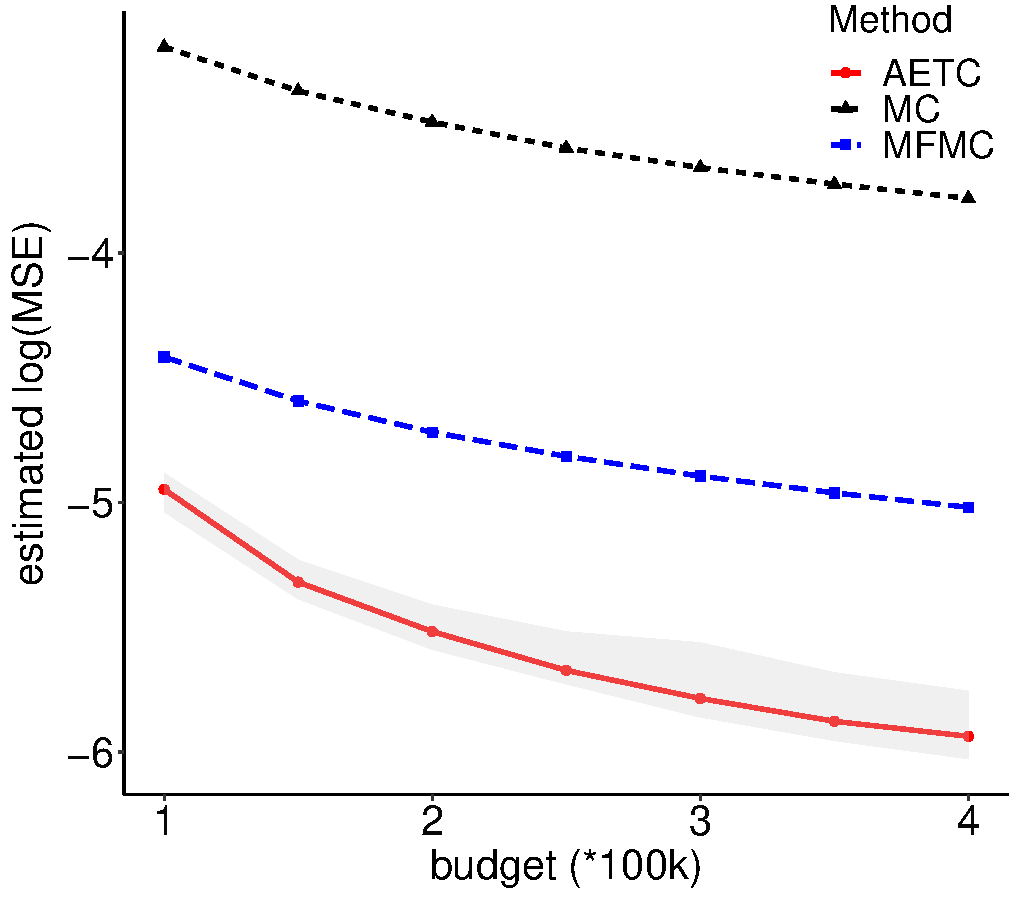
\includegraphics[width=0.30\textwidth]{s-r.pdf}
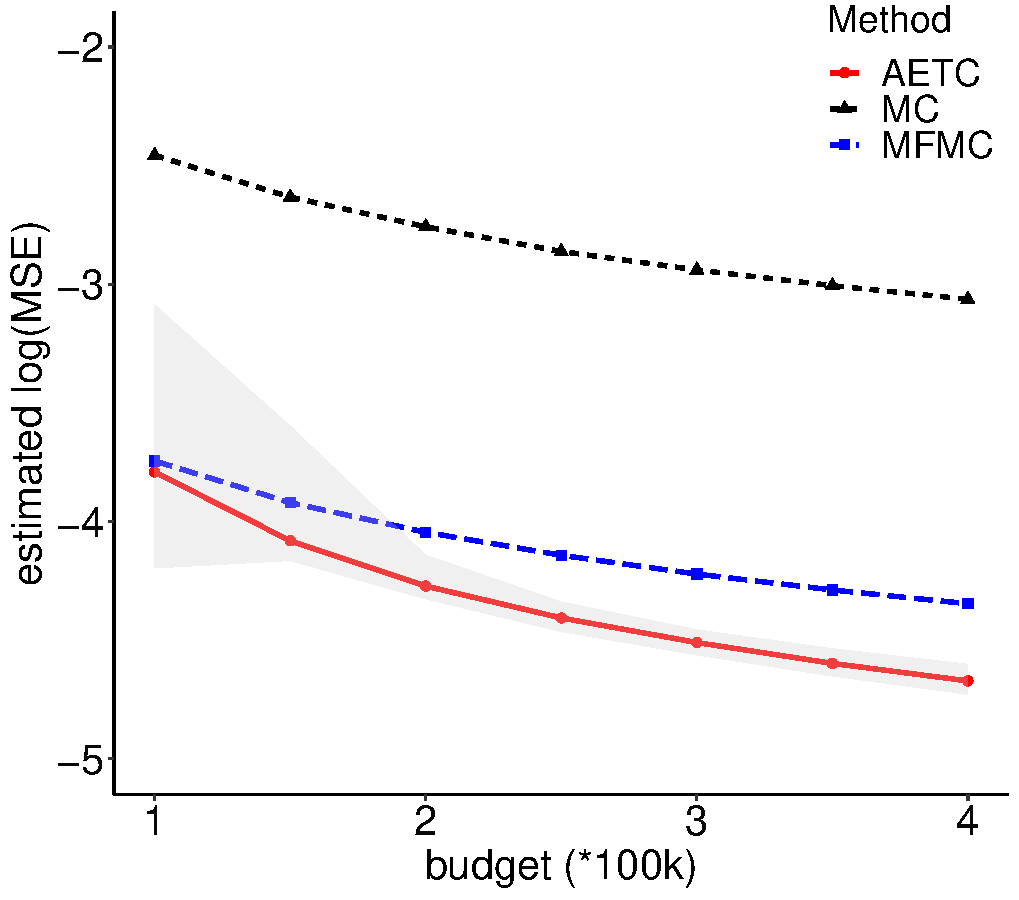
\includegraphics[width=0.30\textwidth]{s-r_new.pdf}
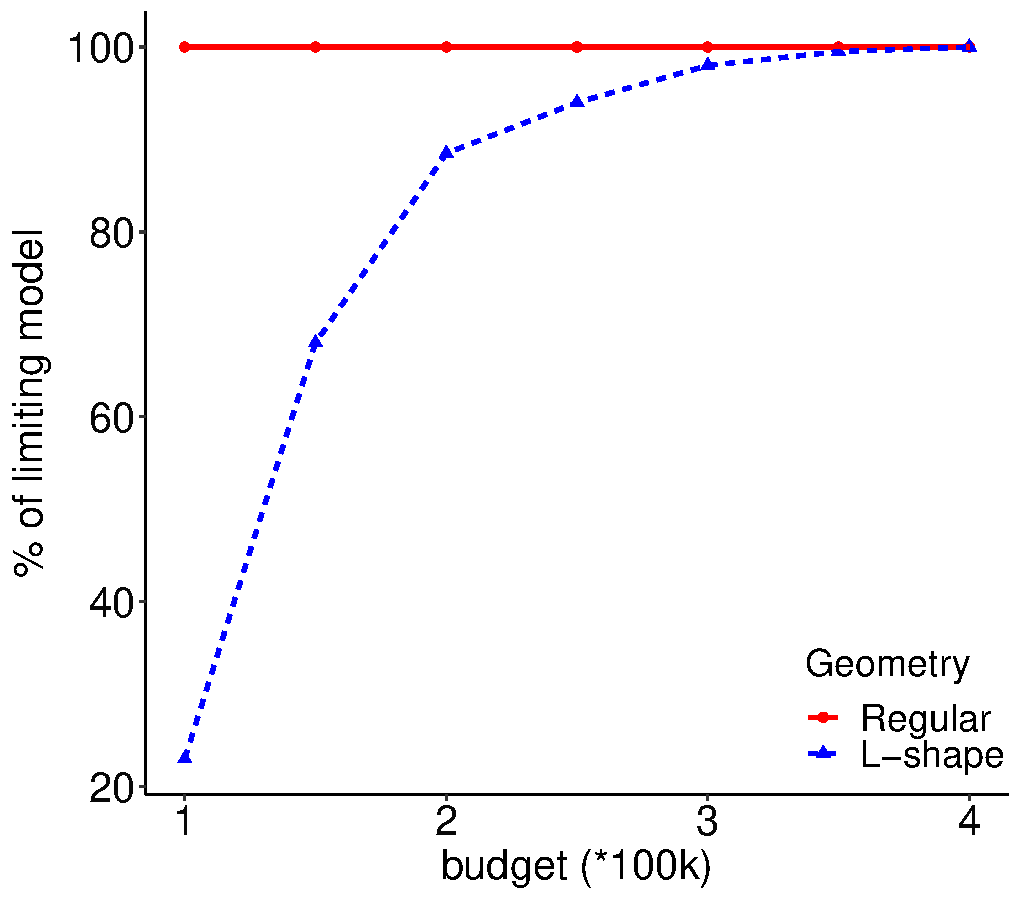
\includegraphics[width=0.30\textwidth]{model_s.pdf}
\caption{\small Comparison of the estimated ($\log_{10}$) mean-squared error of the LRMC estimator given by the AETC algorithm, the Monte Carlo estimator and the Multi-Fidelity Monte-Carlo estimator as budget increases from $10^5$ to $4\times 10^5$ in the case of regular geometry (\textbf{Left}) and $L$-shape geometry (\textbf{Middle}).  In both cases, the $0.05$-$0.50$-$0.95$-quantiles are given for the LRMC estimator to measure the uncertainty. We also plot the percentage of times the AETC algorithm selects the limiting model given by \eqref{min} (\textbf{Right}).}
%The right panel compares the estimated ($\log_{10}$) $Q$-risk of the LRMC estimator given by the AETC algorithm and the Monte Carlo estimator as budget increases from $10^5$ to $4\times 10^5$. In both cases, the $0.05$-$0.50$-$0.95$-quantiles are given for the LRMC estimator to measure the uncertainty. }
  \label{fig:1}
  \end{center}
\end{figure}


The same experiment is repeated when we take $f(Y)$ as multi-dimensional responses. 
Particularly, we take $f(Y)$ as $9$ components of approximate solution.  
For the regular geometry domain, the $9$ components are taken as a randomly selected $3\times 3$ pixel from the $51\times 51$ solution field, while for the $L$-geometry domain, the $9$ components are taken as $9$ randomly selected components from the $2601$-dimensional solution vector (which does not take into account the spatial structure). 
In both cases, the weight matrix $Q$ is set as the identity matrix $R = I_9$, so the regret is the total mean-squared error of the each response. 
We give the oracle information of the correlations between $X^{(i)}$ and $f^{(j)}(Y)$, $i\in [6], j\in [9]$, as in a $9\times 6$ matrix:
\begin{align*}
\small
O_{\text{regular}} = 
\begin{bmatrix}
0.214 &0.165 &0.100 &-0.004 &-0.214&-0.986  \\
0.195&0.146 & 0.078& -0.024&-0.235&-0.990  \\
0.175& 0.124& 0.056& -0.0045&-0.255&-0.991 \\
0.213& 0.163& 0.095& -0.005&-0.216&-0.986  \\
0.193& 0.143& 0.075& -0.026&-0.236&-0.990  \\
0.173& 0.123& 0.055& -0.047&-0.256&-0.991 \\
0.211& 0.161& 0.094& -0.007&-0.218&-0.987 \\
0.191& 0.141& 0.073& -0.028&-0.238&-0.990  \\
0.172& 0.121& 0.053& -0.048&-0.258&-0.991
\end{bmatrix}\\
\\
\small O_{\text{$L$-shape}} = 
\begin{bmatrix}
0.513 &0.528 &0.542&0.520 &0.217 &-0.760 \\
0.722&0.724 & 0.717&0.664& 0.316&-0.824 \\
-0.805& -0.798&-0.776& -0.701& -0.339&0.812 \\
0.533& 0.548& 0.562&0.541& 0.237&-0.781  \\
-0.626& -0.626& -0.616&-0.558& -0.193&0.891  \\
-0.739& -0.740&-0.732& -0.677& -0.330&0.828 \\
0.688& 0.692&0.688& 0.639& 0.293&-0.823 \\
-0.601 &-0.601&-0.592& -0.534& -0.168&0.900  \\
0.690&0.692&0.684& 0.632& 0.282&-0.861
\end{bmatrix},
\end{align*}
where $O_{j,i}$ is the correlation between $X^{(i)}$ and $f^{(j)}(Y)$.  
In both cases, it is clear that the cheapest surrogate model has the highest correlation with all responses, implying that the cost-correlation hierarchical structure (an assumption for the MFMC) is violated. We thus only compare the AETC with the MC. The limiting models expected to be selected by the AETC in both cases are $f(Y)\sim X^{(5)}+X^{(6)}+\text{intercept}$ and $f(Y)\sim X^{(3)}+X^{(4)}+X^{(5)}+X^{(6)}+\text{intercept}$, respectively. The results are given in Figure \ref{fig:11}.

In both Figure \ref{fig:1} and \ref{fig:11}, the AETC algorithm demonstrates a superior performance over the other two methods. Also, as the total budget becomes large, the frequency of the AETC choosing the model given by \eqref{min} converges to $1$, and this verifies our result in Theorem \ref{thm:AETC}. 

\begin{figure}[h!]
\begin{center}
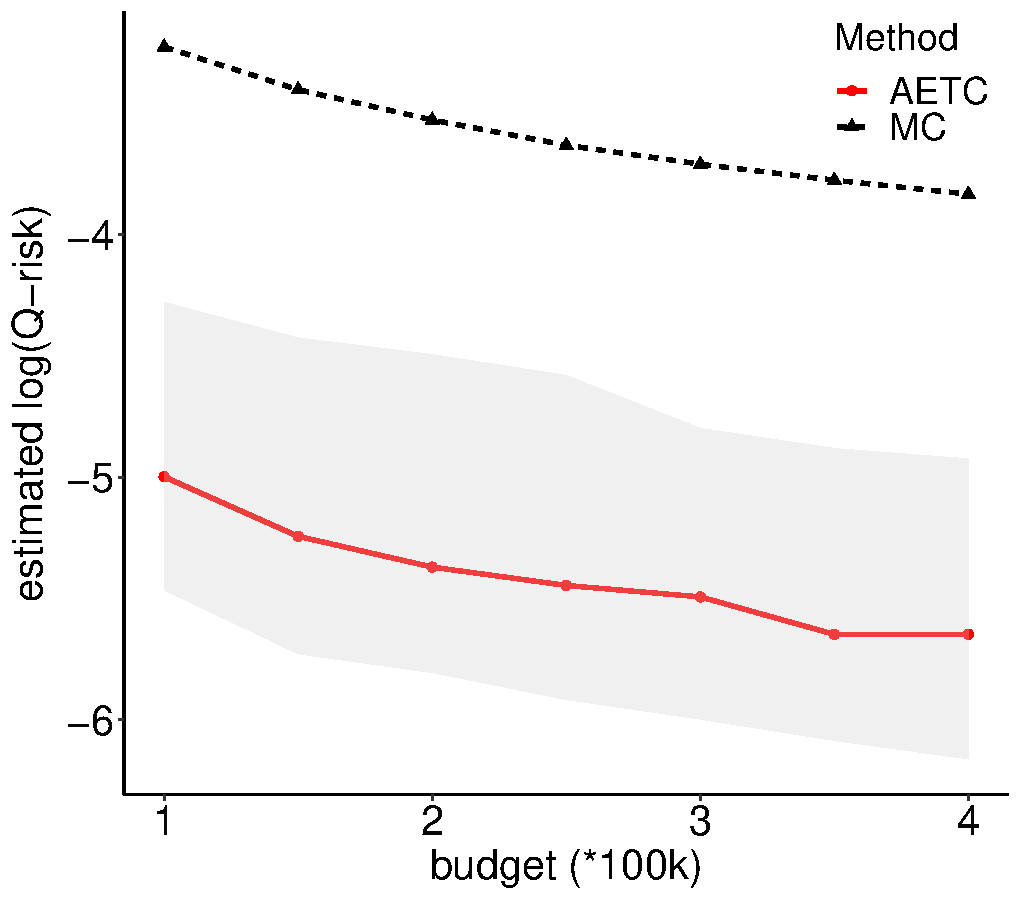
\includegraphics[width=0.30\textwidth]{s-r-m.pdf}
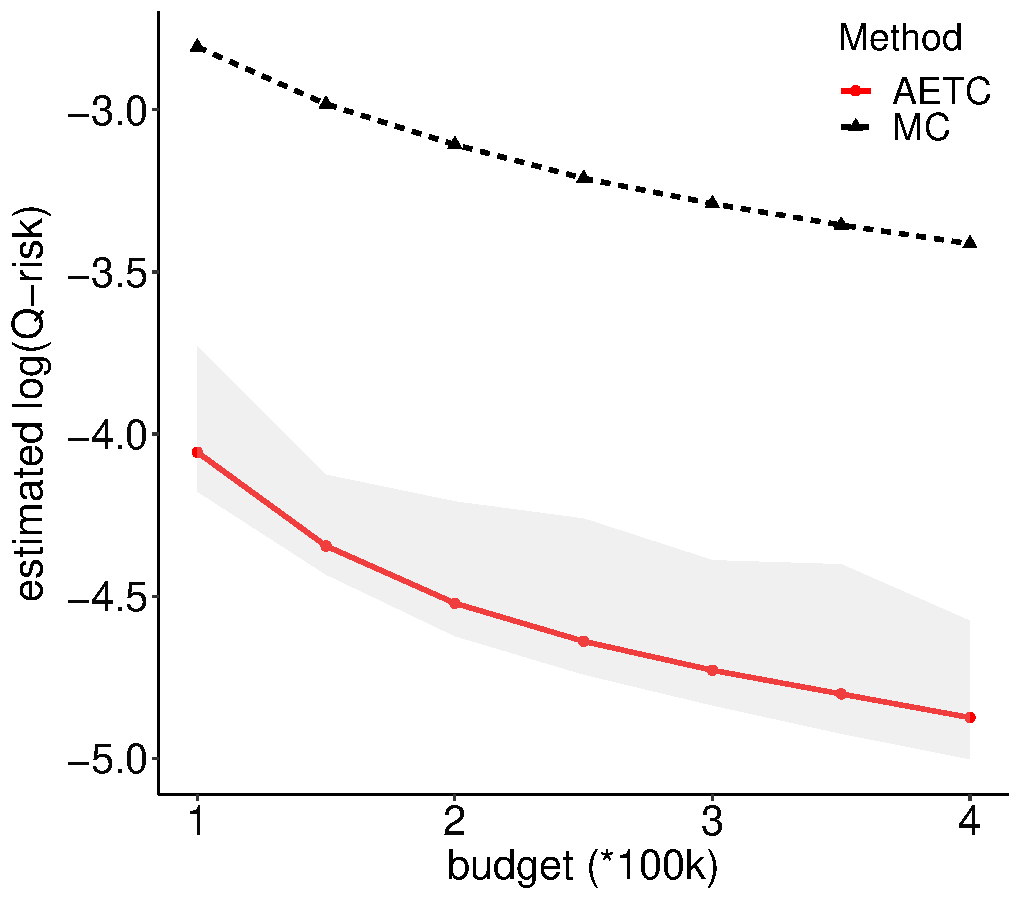
\includegraphics[width=0.30\textwidth]{s-r-m_new.pdf}
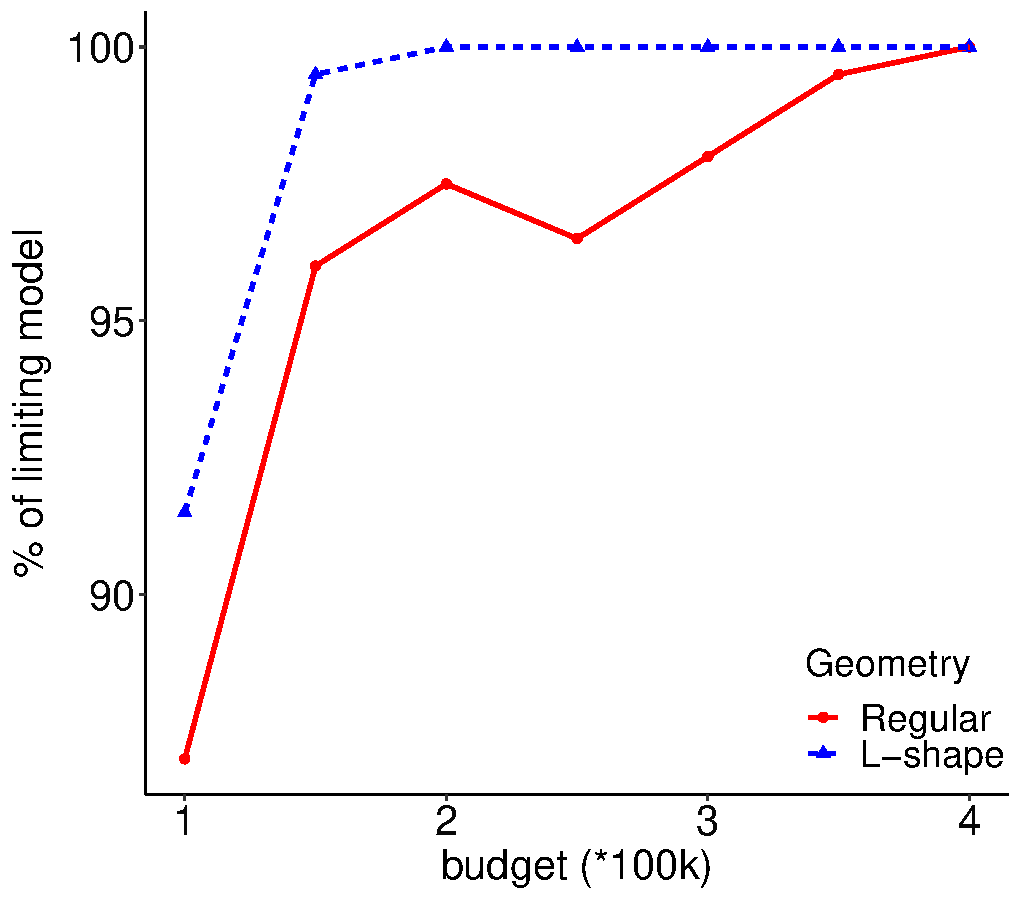
\includegraphics[width=0.30\textwidth]{model_m.pdf}
\caption{\small Comparison of the estimated ($\log_{10}$) $Q$-risk of the LRMC estimator given by the AETC algorithm, the Monte Carlo estimator and the Multi-Fidelity Monte-Carlo estimator as budget increases from $10^5$ to $4\times 10^5$ in the case of regular geometry (\textbf{Left}) and $L$-shape geometry (\textbf{Middle}).  In both cases, the $0.05$-$0.50$-$0.95$-quantiles are given for the LRMC estimator to measure the uncertainty. We also plot the percentage of times the AETC algorithm selects the limiting model given by \eqref{min} (\textbf{Right}).}
  \label{fig:11}
  \end{center}
\end{figure}

We now test the AETC algorithm in large-scale approximation. 
Fix the budget as $B = 4\times 10^5$, and let $f(Y) = u^{(0)}\in\R^{2601}$ be the approximate solution given by the highest-fidelity model.  
In this case, the number of affordable samples by the MC is $\lfloor B/4096\rfloor = 97$. 
We now use both the AETC and MC algorithms to compute $\E[f(Y)]$. 
In our experiment, the exploration round $m$ chosen by the AETC in the case of regular geometry and $L$-shape geometry is $60$ and $26$, respectively.
The respective models for exploitation are $f(Y)\sim X^{(5)}+X^{(6)}+\text{intercept}$ and $f(Y)\sim X^{(3)}+X^{(4)}+X^{(5)}+X^{(6)}+\text{intercept}$, and the affordable samples are $14468$ and $3035$. The estimated values and estimation errors are compared to the MC algorithm in Figure \ref{fig:2}. 
\begin{figure}[h!]
\begin{center}
  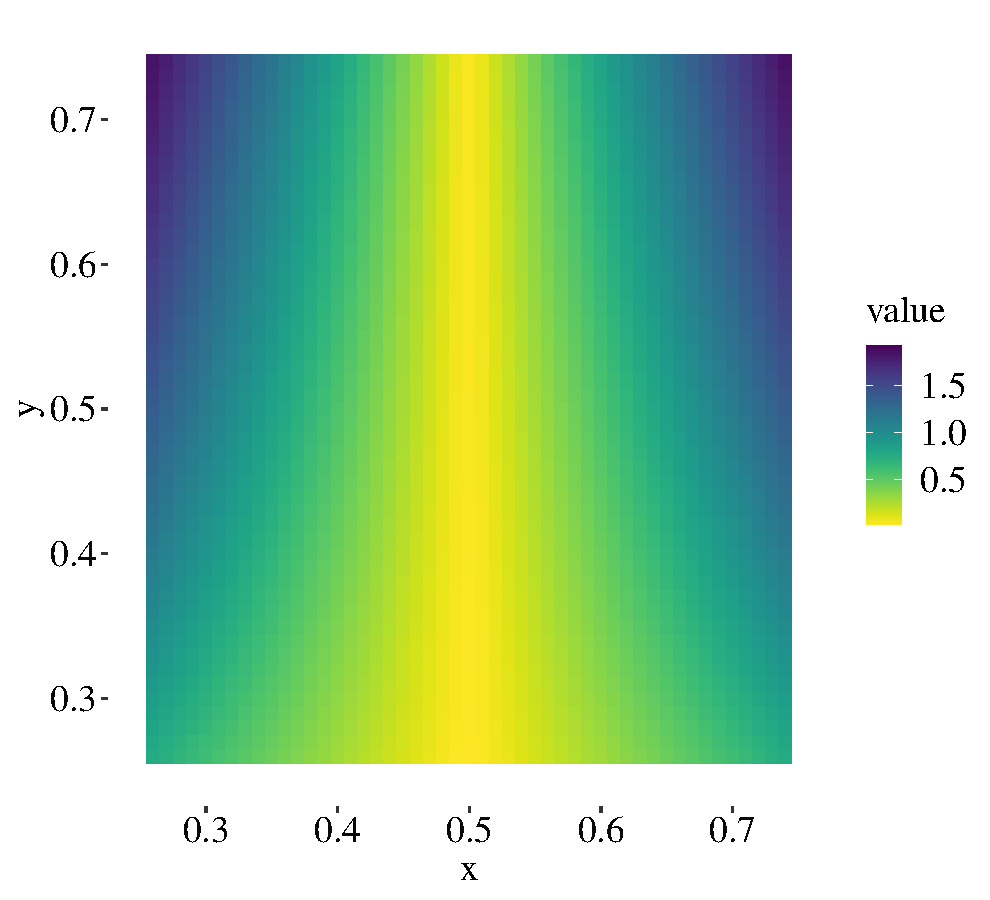
\includegraphics[width=0.328\textwidth]{r.pdf}
  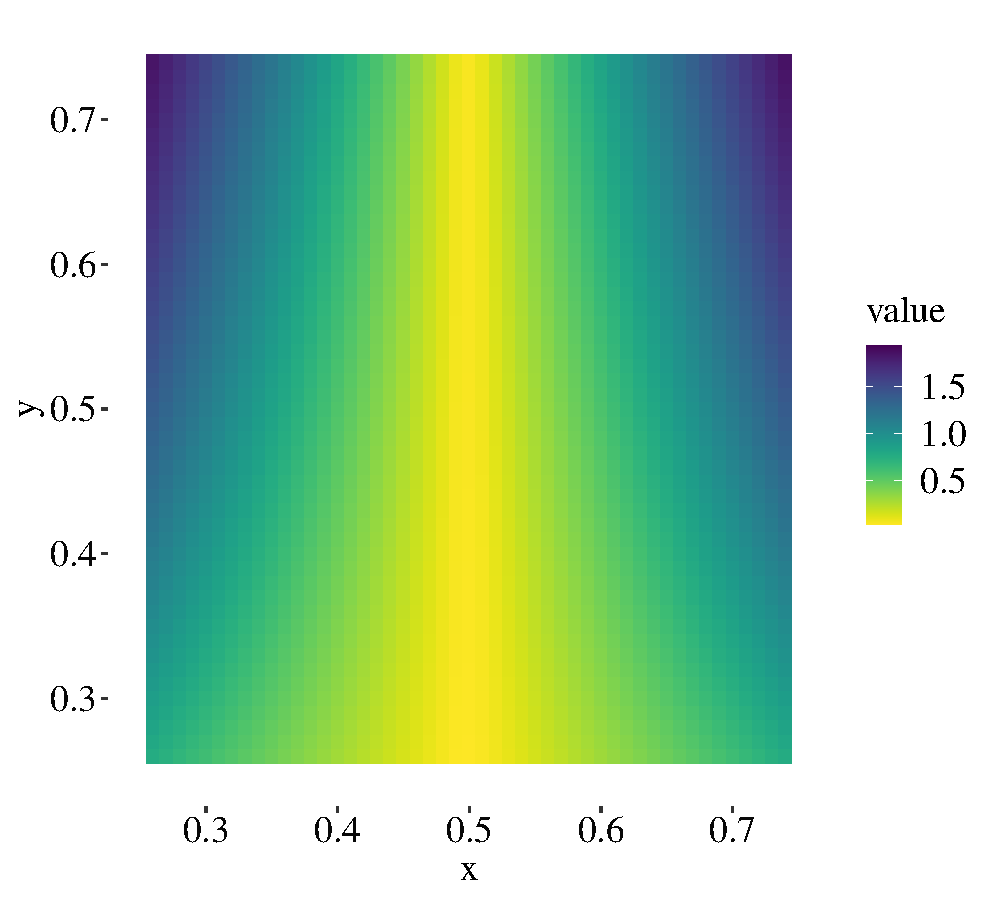
\includegraphics[width=0.328\textwidth]{r_mc.pdf}
   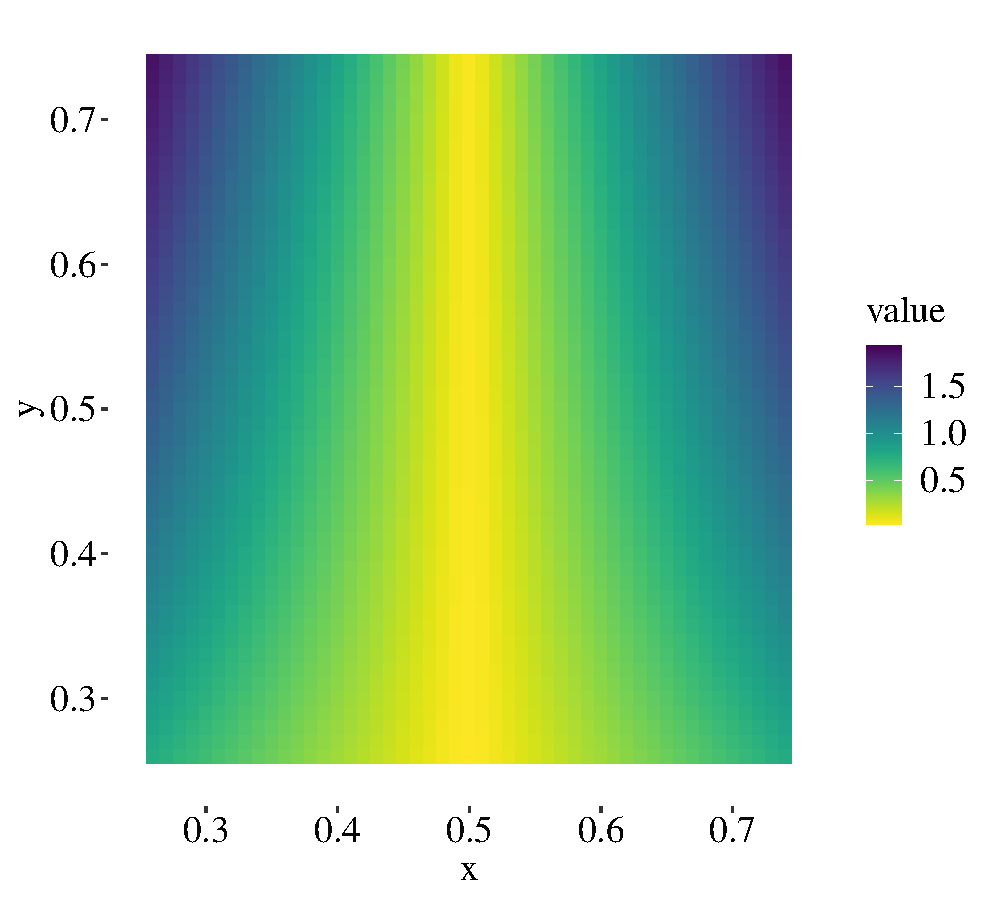
\includegraphics[width=0.328\textwidth]{r_lrmc.pdf}
     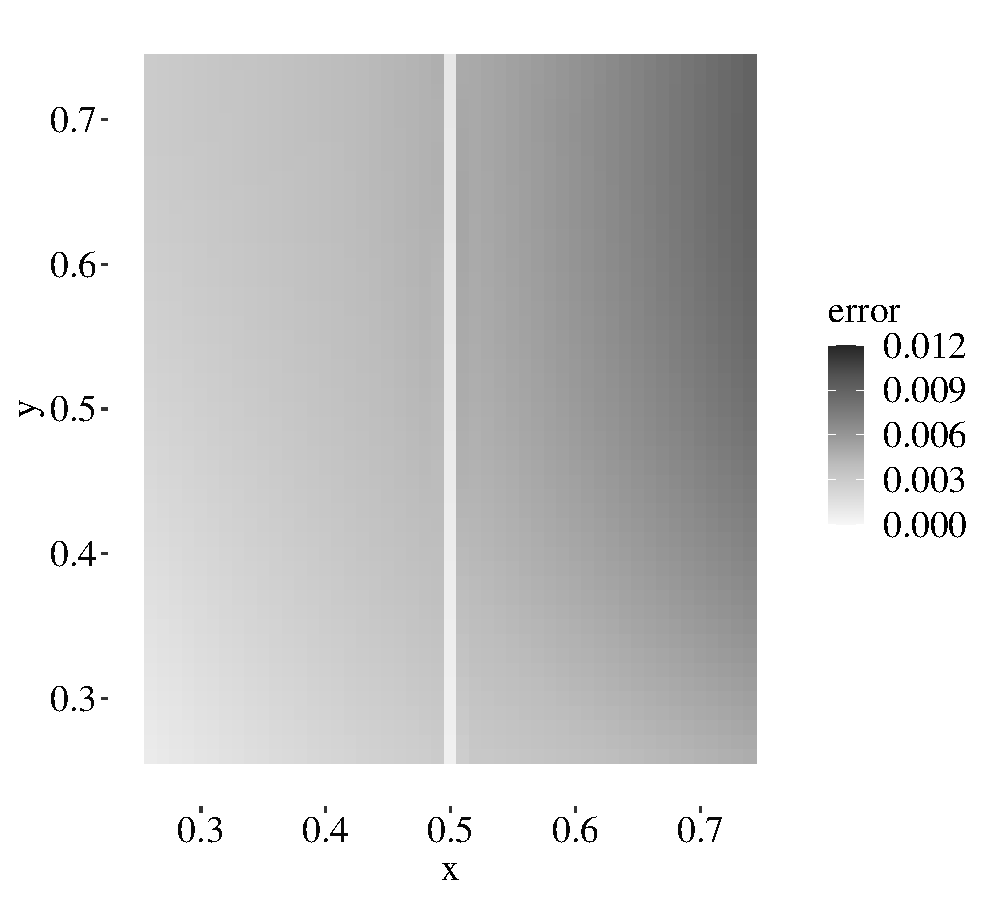
\includegraphics[width=0.34\textwidth]{error_mc.pdf}\ \ \ \ \
  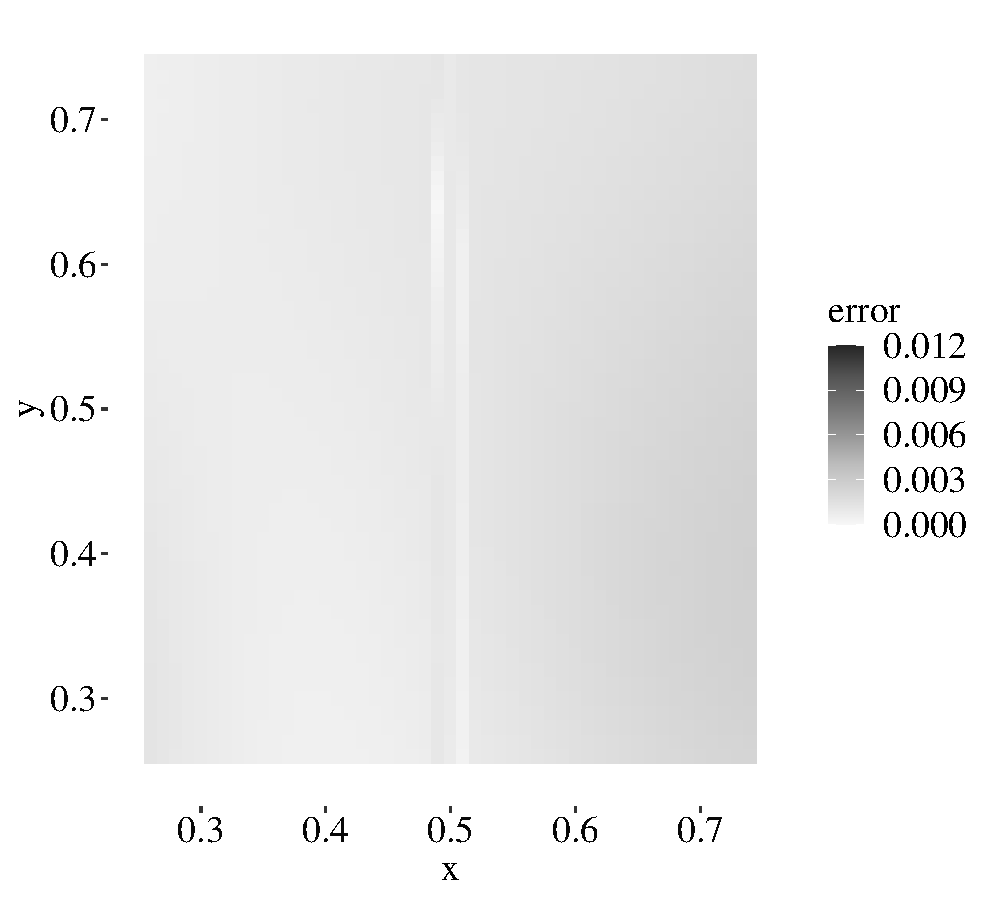
\includegraphics[width=0.34\textwidth]{error_lrmc.pdf}
  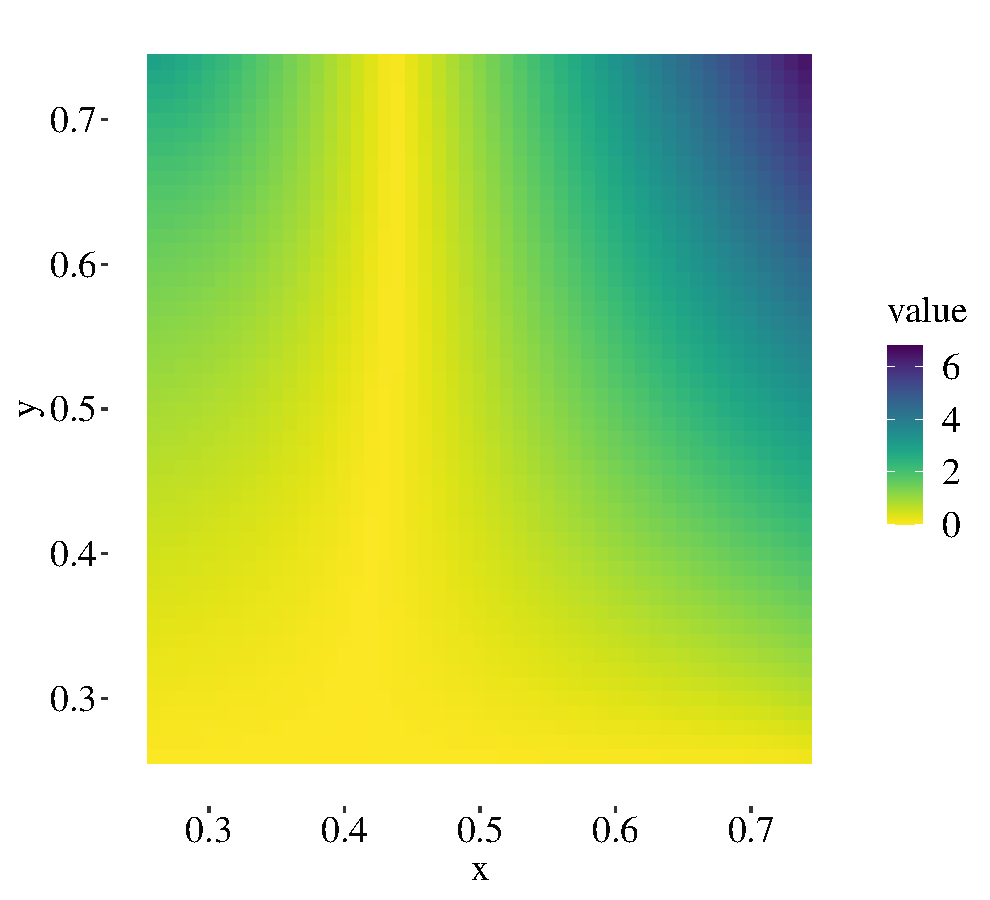
\includegraphics[width=0.328\textwidth]{r_new.pdf}
  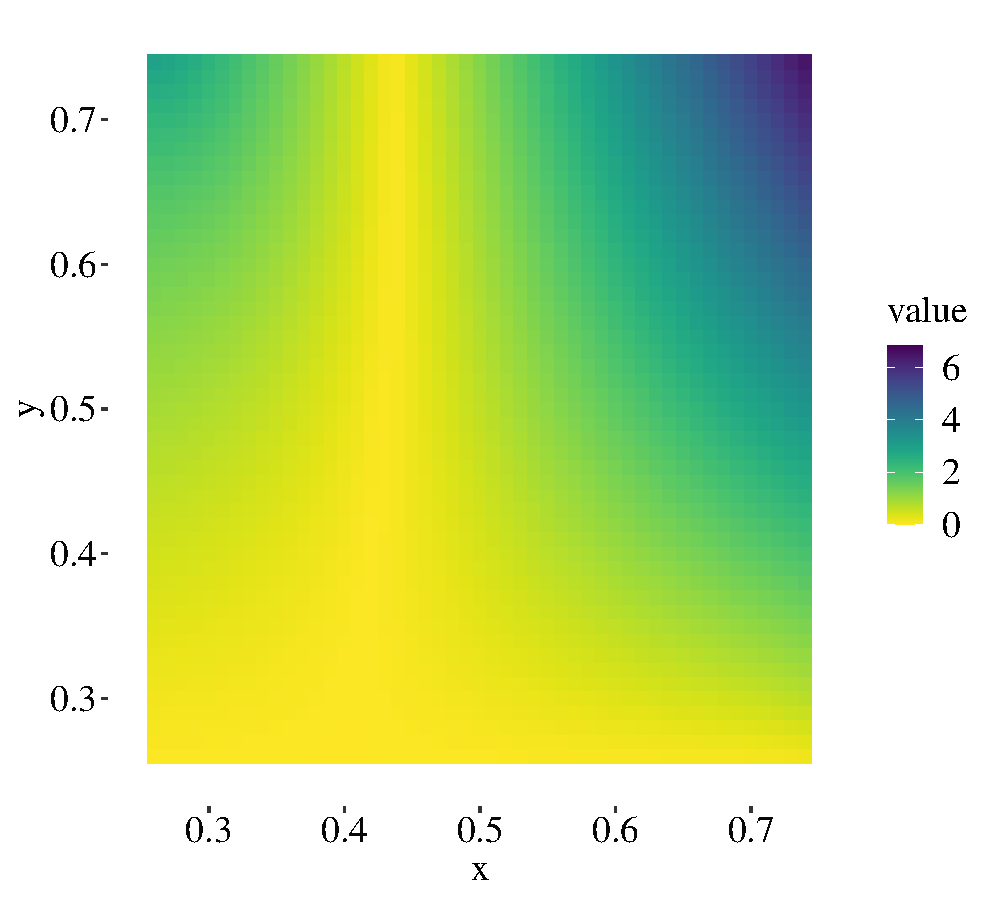
\includegraphics[width=0.328\textwidth]{r_mc_new.pdf}
   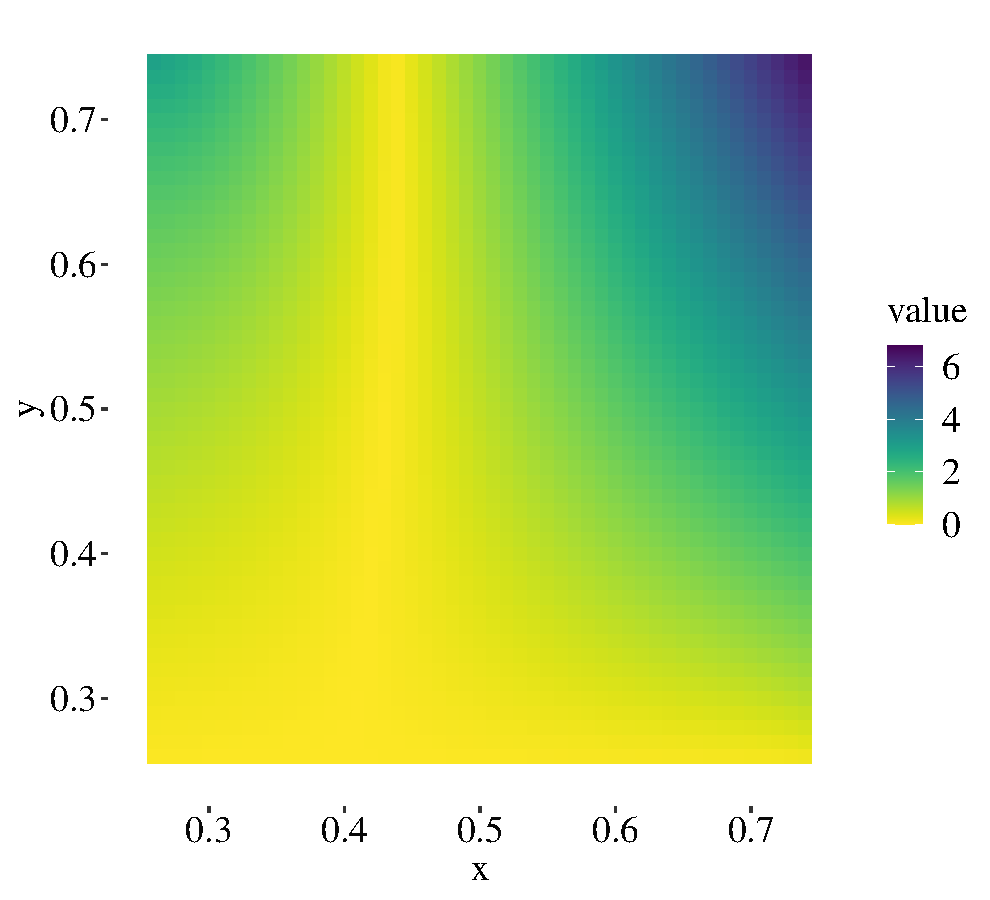
\includegraphics[width=0.328\textwidth]{r_lrmc_new.pdf}
     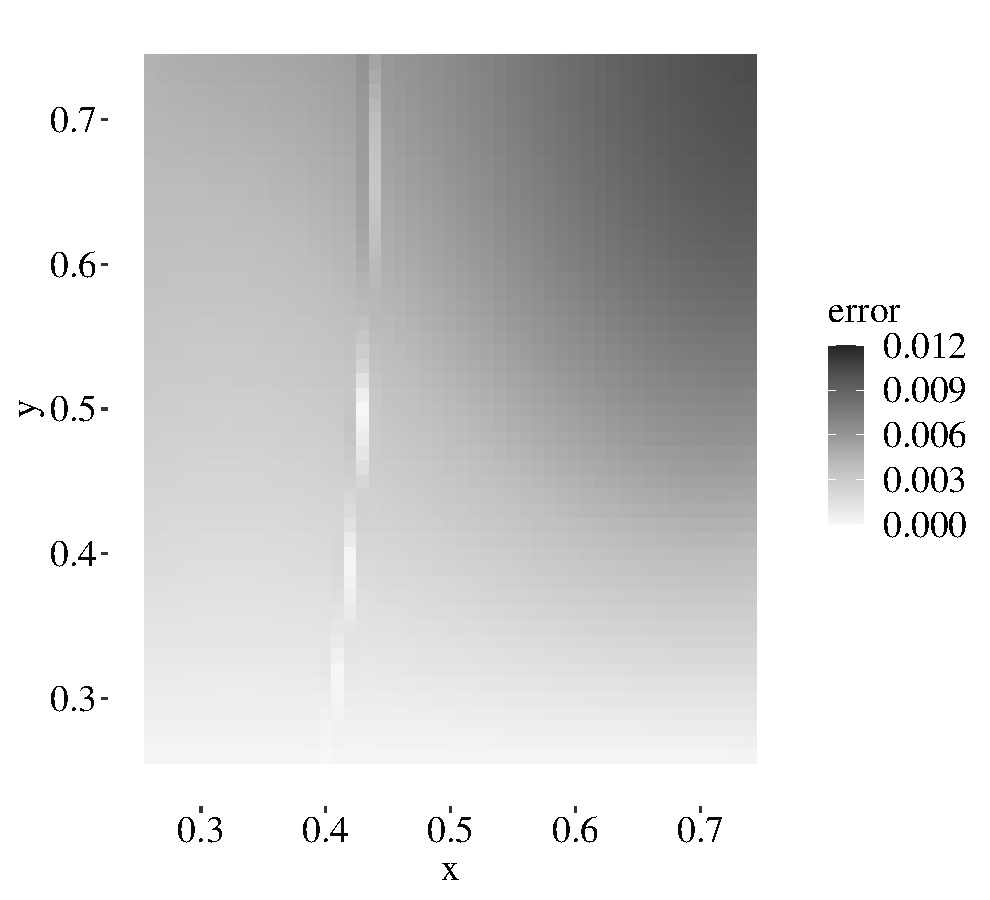
\includegraphics[width=0.34\textwidth]{error_mc_new.pdf}\ \ \ \ \ 
  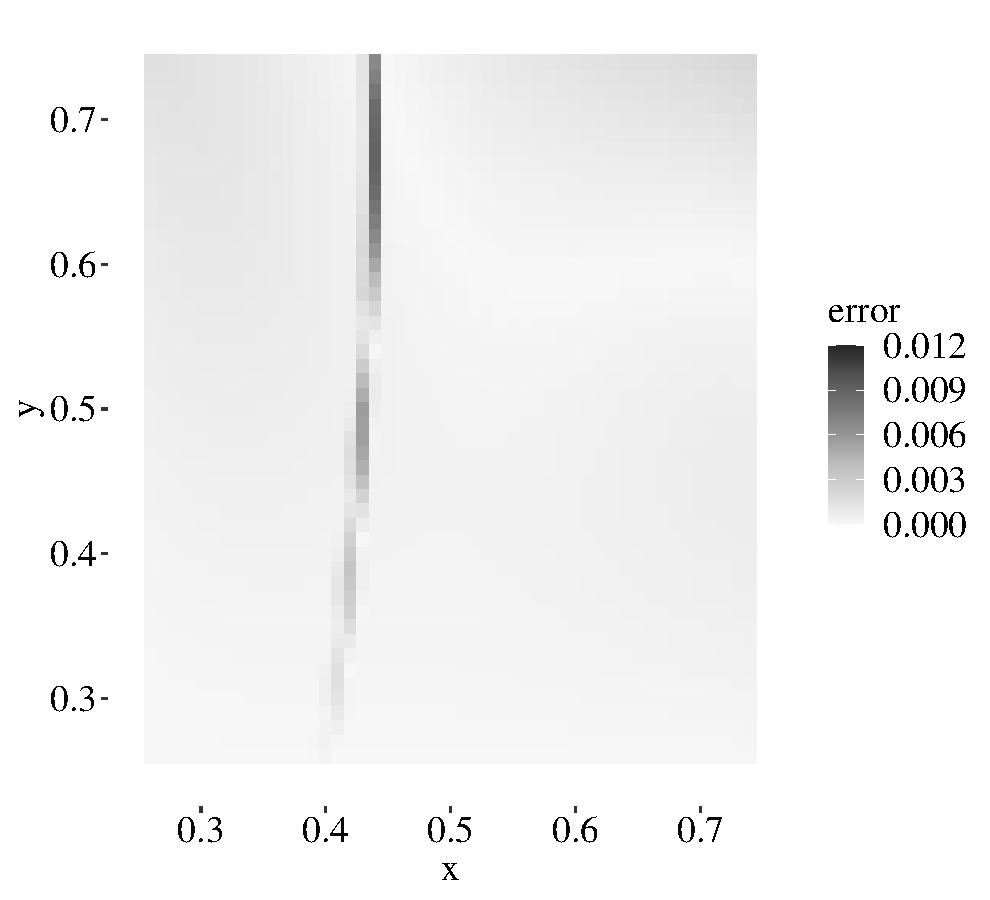
\includegraphics[width=0.34\textwidth]{error_lrmc_new.pdf}
  \caption{\small Comparison of the estimated $\E[f(X)]$ by the AETC and MC algorithms. The top and bottom panels are the results for the regular geometry and $L$-shape geometry, respectively. 
In each panel, $\E[f(X)]$ estimated from the MC (\textbf{Middle}) and the AETC (\textbf{Right}) is compared to the ground truth (\textbf{Left}), which is calculated by averaging $50000$ independent samples using the MC. To better compare the estimation errors, we compute the absolute value of the difference between the estimated $\E[Y]$ and the ground truth for each component in $\E[f(Y)]$. The plot on the left and right corresponds to the errors committed by MC and AETC, respectively.}
  \label{fig:2}
  \end{center}
\end{figure}



%\begin{figure}[h!]
%\centering
%   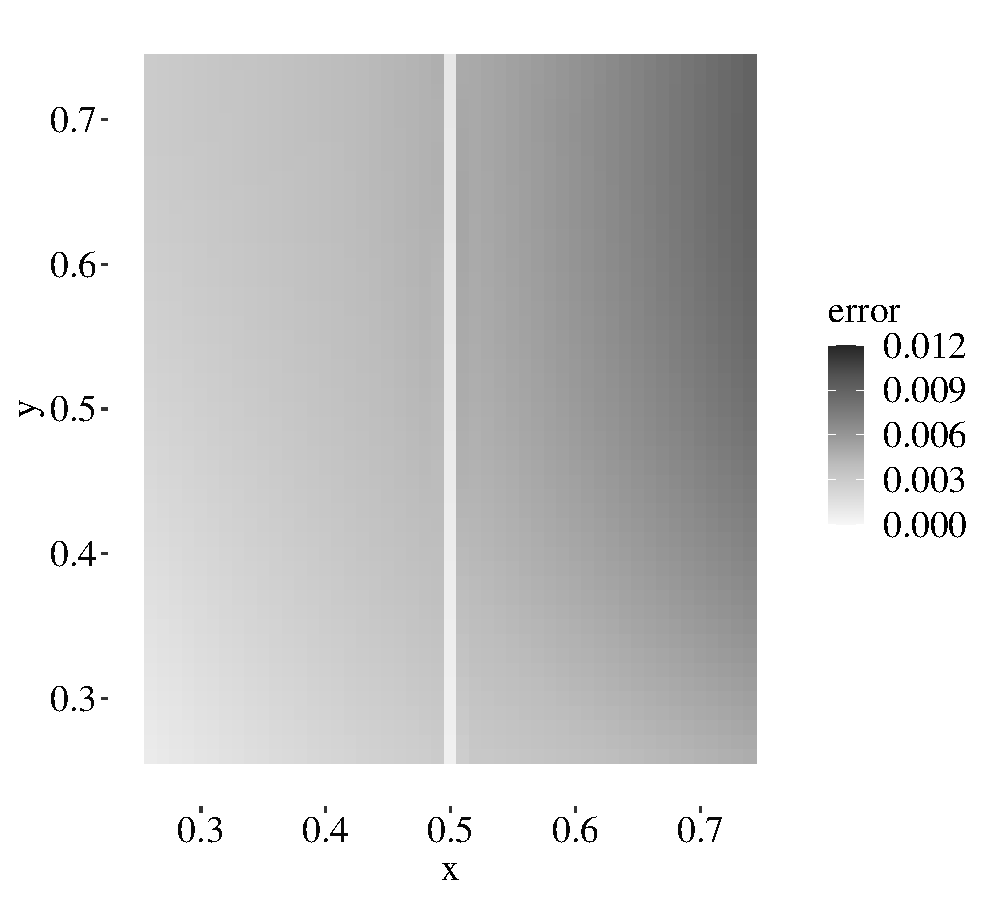
\includegraphics[width=0.35\textwidth]{error_mc.pdf}
%  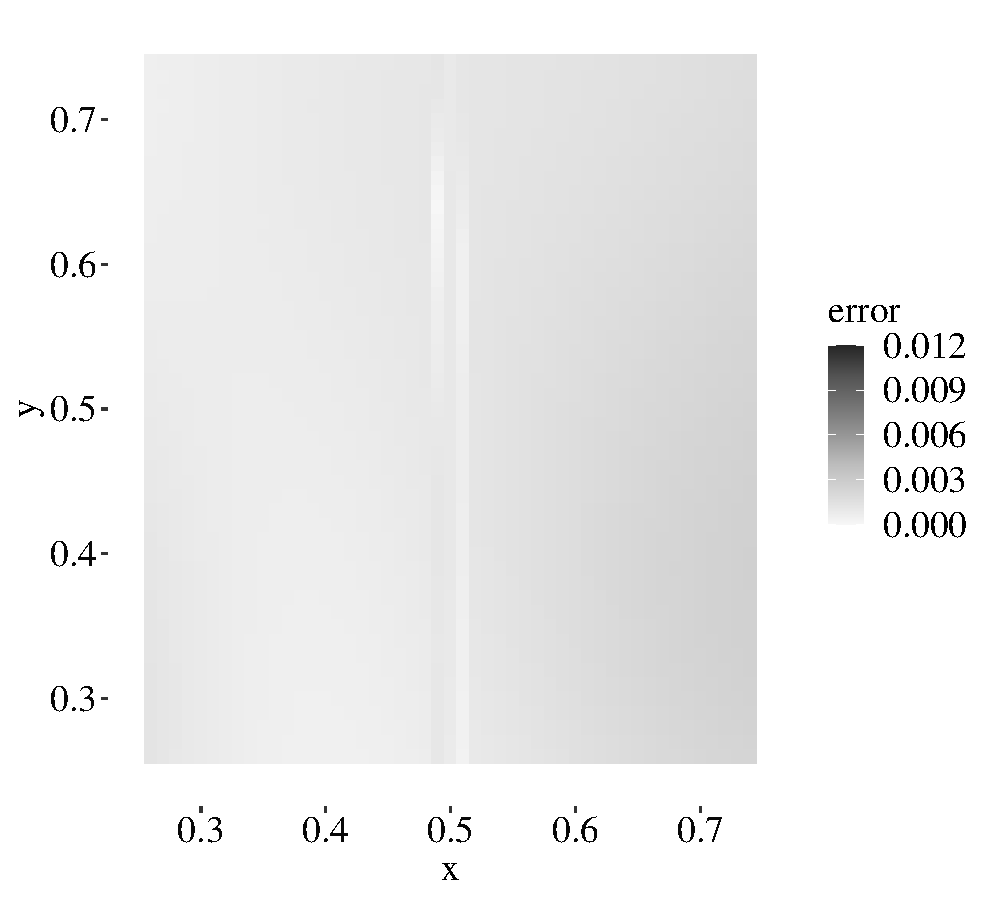
\includegraphics[width=0.35\textwidth]{error_lrmc.pdf}
%  \caption{\small Estimation error of the MC (left) and AETC (right) algorithms compared to the ground truth.}
%  \label{fig:3}
%\end{figure}


\printbibliography

\end{document}